\section{findscreen Class Reference}
\label{classfindscreen}\index{findscreen@{findscreen}}
{\tt \#include $<$findscreen.h$>$}

Collaboration diagram for findscreen:\begin{figure}[H]
\begin{center}
\leavevmode
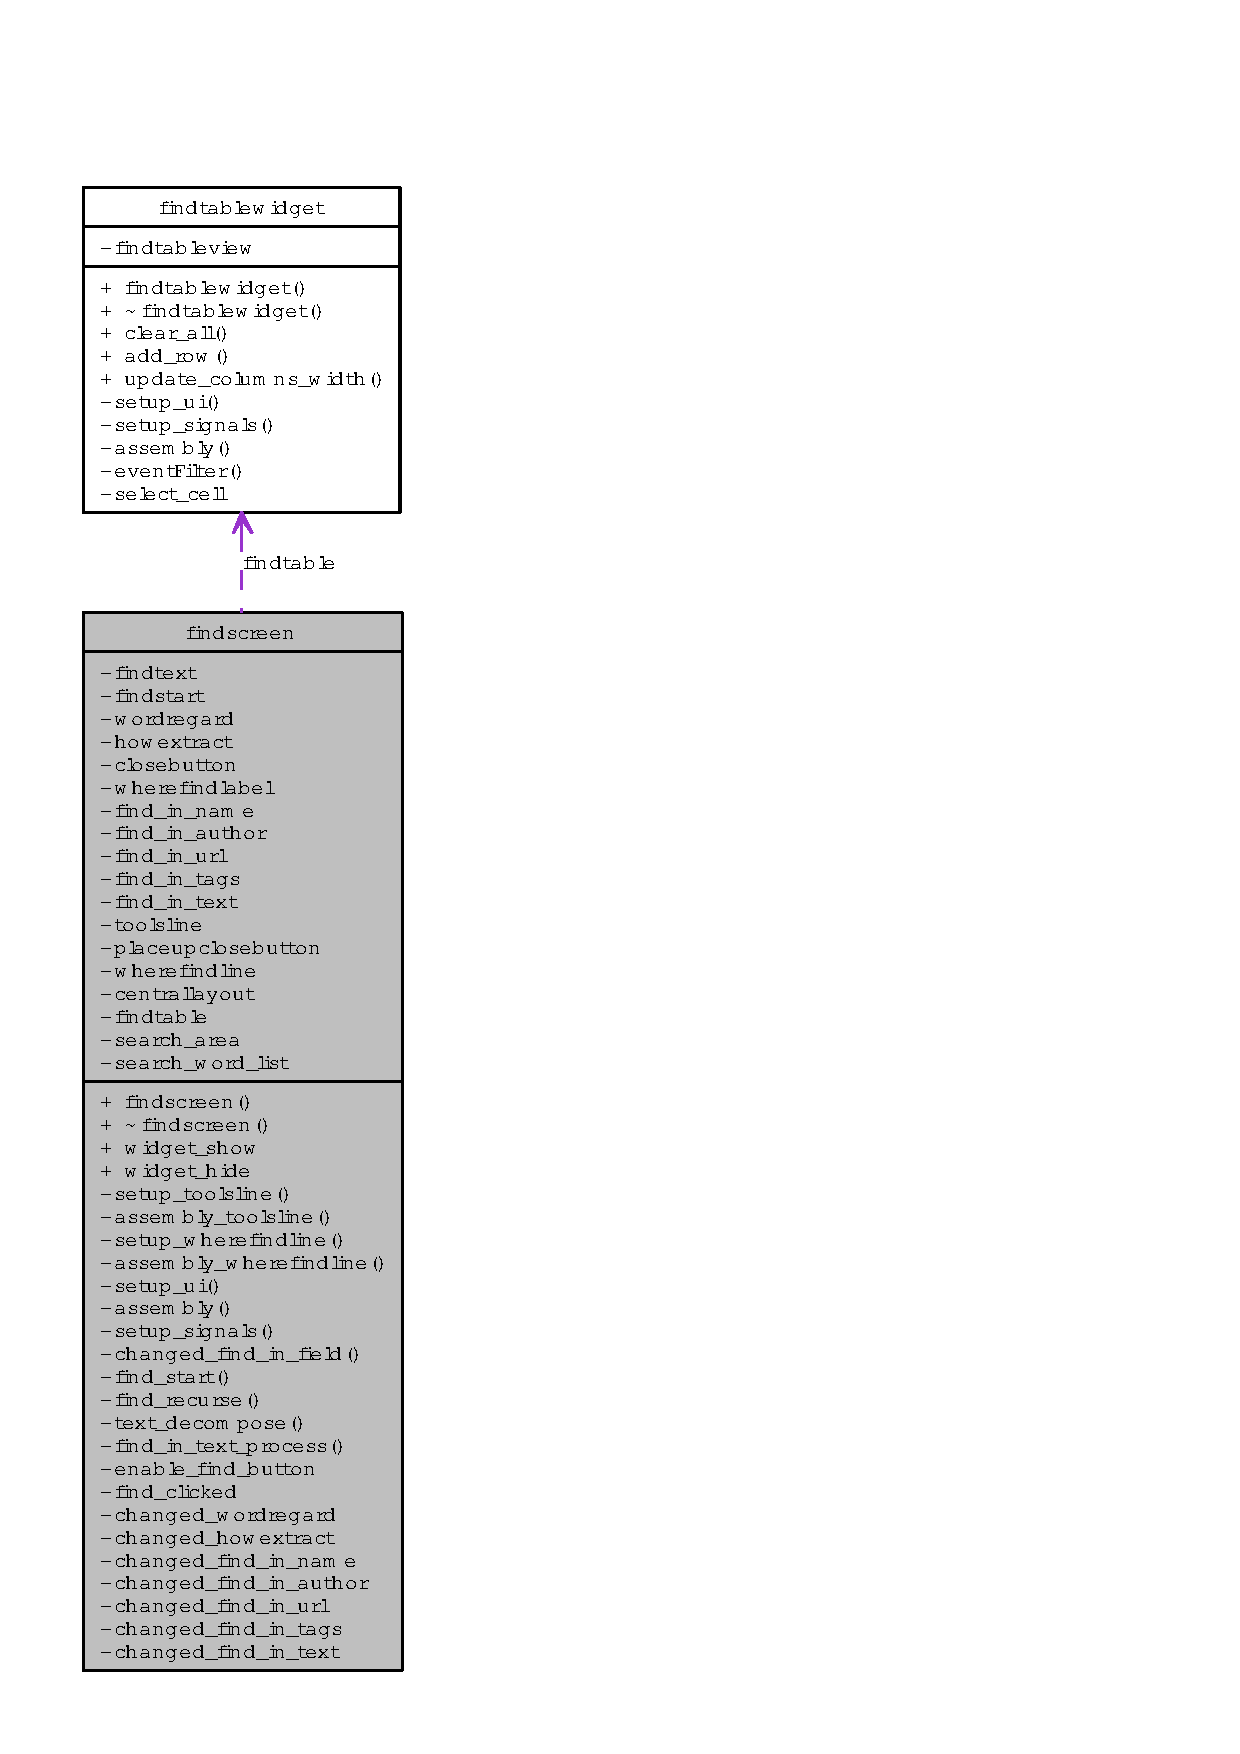
\includegraphics[width=98pt]{classfindscreen__coll__graph}
\end{center}
\end{figure}
\subsection*{Public Slots}
\begin{CompactItemize}
\item 
void {\bf widget\_\-show} (void)
\item 
void {\bf widget\_\-hide} (void)
\end{CompactItemize}
\subsection*{Public Member Functions}
\begin{CompactItemize}
\item 
{\bf findscreen} (QWidget $\ast$parent=0)
\item 
virtual {\bf $\sim$findscreen} (void)
\end{CompactItemize}
\subsection*{Private Slots}
\begin{CompactItemize}
\item 
void {\bf enable\_\-find\_\-button} (const QString \&text)
\item 
void {\bf find\_\-clicked} (void)
\item 
void {\bf changed\_\-wordregard} (int pos)
\item 
void {\bf changed\_\-howextract} (int pos)
\item 
void {\bf changed\_\-find\_\-in\_\-name} (int state)
\item 
void {\bf changed\_\-find\_\-in\_\-author} (int state)
\item 
void {\bf changed\_\-find\_\-in\_\-url} (int state)
\item 
void {\bf changed\_\-find\_\-in\_\-tags} (int state)
\item 
void {\bf changed\_\-find\_\-in\_\-text} (int state)
\end{CompactItemize}
\subsection*{Private Member Functions}
\begin{CompactItemize}
\item 
void {\bf setup\_\-toolsline} (void)
\item 
void {\bf assembly\_\-toolsline} (void)
\item 
void {\bf setup\_\-wherefindline} (void)
\item 
void {\bf assembly\_\-wherefindline} (void)
\item 
void {\bf setup\_\-ui} (void)
\item 
void {\bf assembly} (void)
\item 
void {\bf setup\_\-signals} (void)
\item 
void {\bf changed\_\-find\_\-in\_\-field} (QString fieldname, int state)
\item 
void {\bf find\_\-start} (void)
\item 
void {\bf find\_\-recurse} ({\bf Tree\-Item} $\ast$curritem)
\item 
QString\-List {\bf text\_\-decompose} (QString text)
\item 
bool {\bf find\_\-in\_\-text\_\-process} (const QString \&text)
\end{CompactItemize}
\subsection*{Private Attributes}
\begin{CompactItemize}
\item 
QLine\-Edit $\ast$ {\bf findtext}
\item 
QPush\-Button $\ast$ {\bf findstart}
\item 
QCombo\-Box $\ast$ {\bf wordregard}
\item 
QCombo\-Box $\ast$ {\bf howextract}
\item 
QTool\-Button $\ast$ {\bf closebutton}
\item 
QLabel $\ast$ {\bf wherefindlabel}
\item 
QCheck\-Box $\ast$ {\bf find\_\-in\_\-name}
\item 
QCheck\-Box $\ast$ {\bf find\_\-in\_\-author}
\item 
QCheck\-Box $\ast$ {\bf find\_\-in\_\-url}
\item 
QCheck\-Box $\ast$ {\bf find\_\-in\_\-tags}
\item 
QCheck\-Box $\ast$ {\bf find\_\-in\_\-text}
\item 
QHBox\-Layout $\ast$ {\bf toolsline}
\item 
QVBox\-Layout $\ast$ {\bf placeupclosebutton}
\item 
QHBox\-Layout $\ast$ {\bf wherefindline}
\item 
QVBox\-Layout $\ast$ {\bf centrallayout}
\item 
{\bf findtablewidget} $\ast$ {\bf findtable}
\item 
QMap$<$ QString, bool $>$ {\bf search\_\-area}
\item 
QString\-List {\bf search\_\-word\_\-list}
\end{CompactItemize}


\subsection{Detailed Description}




Definition at line 21 of file findscreen.h.

\subsection{Constructor \& Destructor Documentation}
\index{findscreen@{findscreen}!findscreen@{findscreen}}
\index{findscreen@{findscreen}!findscreen@{findscreen}}
\subsubsection{\setlength{\rightskip}{0pt plus 5cm}findscreen::findscreen (QWidget $\ast$ {\em parent} = {\tt 0})}\label{classfindscreen_642becd9c3569e1e9aacfdb96d693dcf}




Definition at line 21 of file findscreen.cpp.

References assembly(), assembly\_\-toolsline(), assembly\_\-wherefindline(), setup\_\-signals(), setup\_\-toolsline(), setup\_\-ui(), and setup\_\-wherefindline().

Here is the call graph for this function:\begin{figure}[H]
\begin{center}
\leavevmode
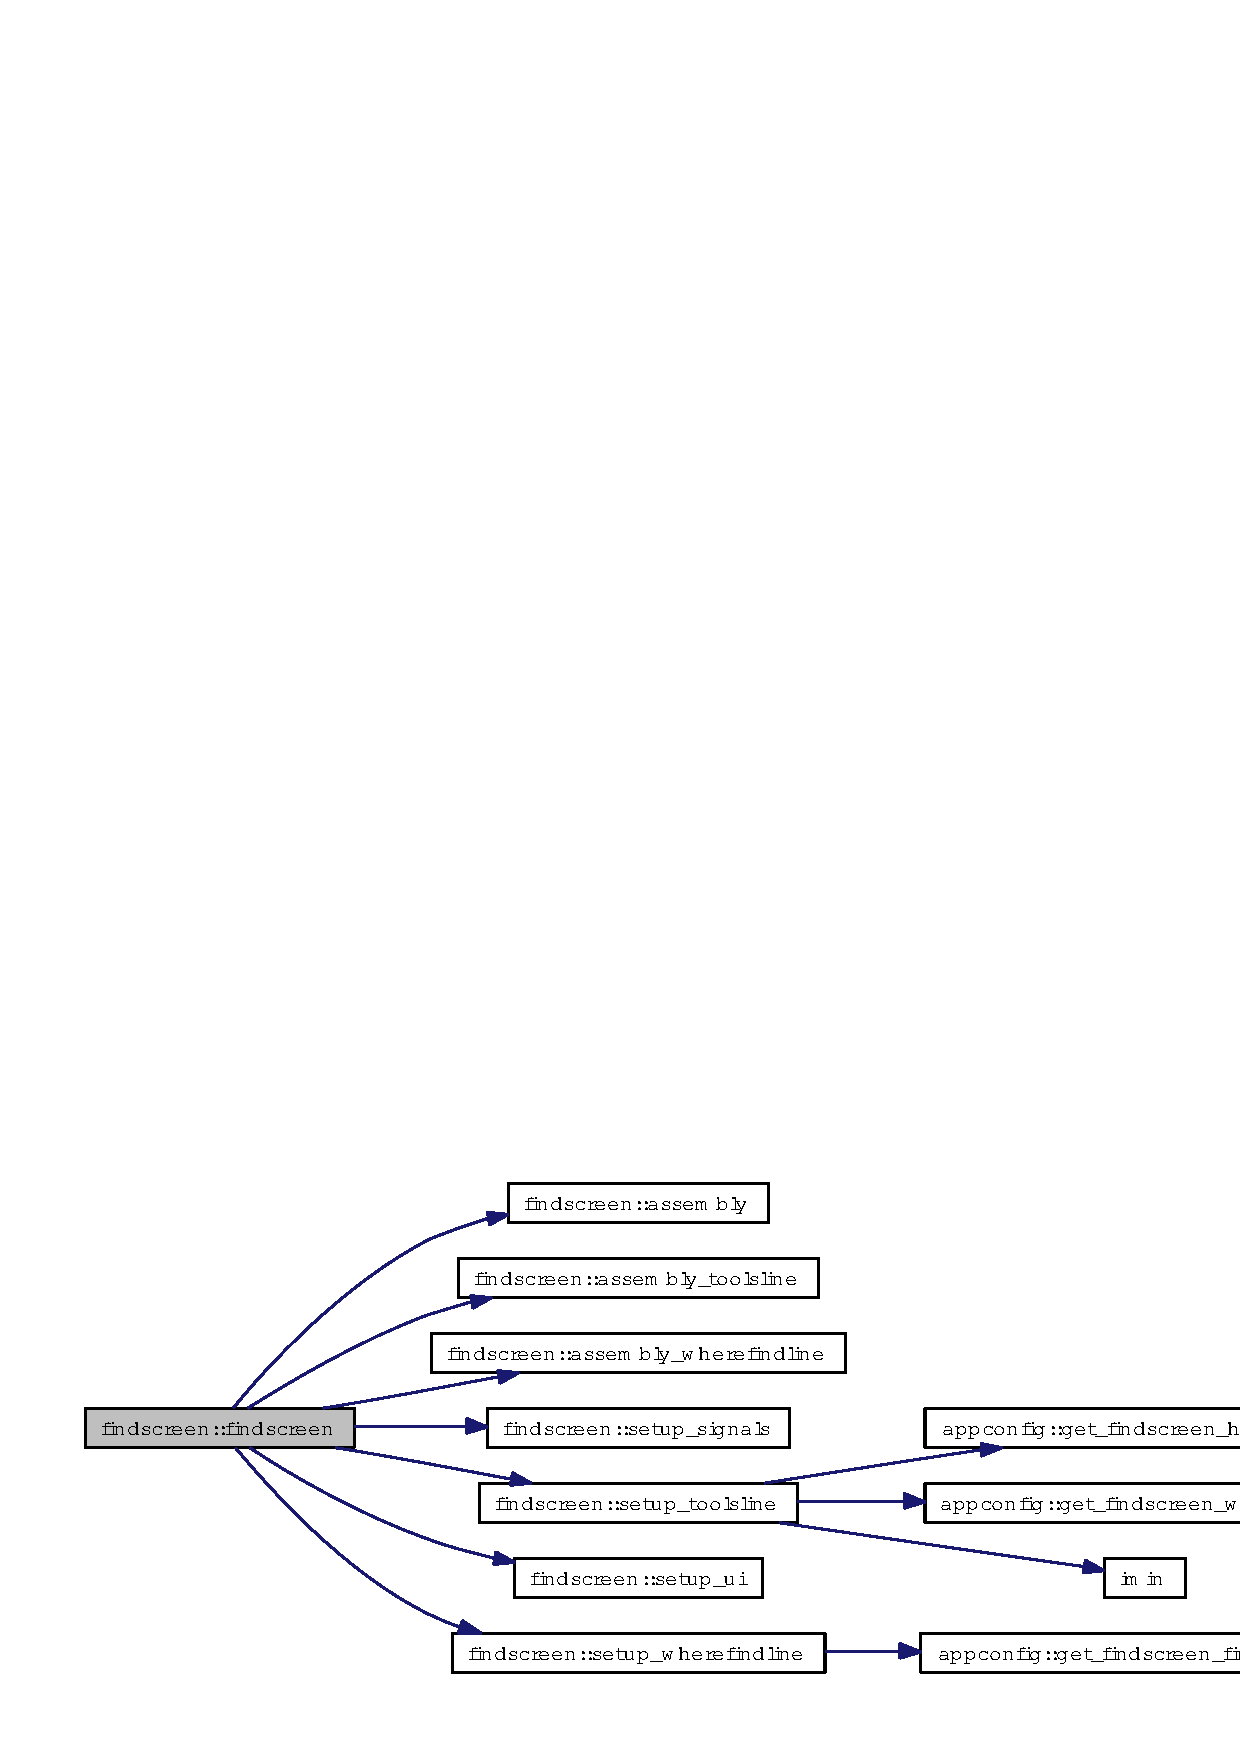
\includegraphics[width=330pt]{classfindscreen_642becd9c3569e1e9aacfdb96d693dcf_cgraph}
\end{center}
\end{figure}
\index{findscreen@{findscreen}!~findscreen@{$\sim$findscreen}}
\index{~findscreen@{$\sim$findscreen}!findscreen@{findscreen}}
\subsubsection{\setlength{\rightskip}{0pt plus 5cm}findscreen::$\sim$findscreen (void)\hspace{0.3cm}{\tt  [virtual]}}\label{classfindscreen_4165198100ade50addc48b0734d93c93}




Definition at line 36 of file findscreen.cpp.

\subsection{Member Function Documentation}
\index{findscreen@{findscreen}!widget_show@{widget\_\-show}}
\index{widget_show@{widget\_\-show}!findscreen@{findscreen}}
\subsubsection{\setlength{\rightskip}{0pt plus 5cm}void findscreen::widget\_\-show (void)\hspace{0.3cm}{\tt  [slot]}}\label{classfindscreen_90ec8cf049de60964e6f0037f8bb9eb4}




Definition at line 467 of file findscreen.cpp.

References mytetraconfig, and appconfig::set\_\-findscreen\_\-show().

Referenced by recordtablescreen::findinbase\_\-open().\index{findscreen@{findscreen}!widget_hide@{widget\_\-hide}}
\index{widget_hide@{widget\_\-hide}!findscreen@{findscreen}}
\subsubsection{\setlength{\rightskip}{0pt plus 5cm}void findscreen::widget\_\-hide (void)\hspace{0.3cm}{\tt  [slot]}}\label{classfindscreen_42187bda0c53a3dbc227da053ce000de}




Definition at line 474 of file findscreen.cpp.

References mytetraconfig, appconfig::set\_\-findscreen\_\-show(), and appconfig::set\_\-findsplitter\_\-size\_\-list().

Referenced by recordtablescreen::findinbase\_\-open(), and setup\_\-signals().\index{findscreen@{findscreen}!enable_find_button@{enable\_\-find\_\-button}}
\index{enable_find_button@{enable\_\-find\_\-button}!findscreen@{findscreen}}
\subsubsection{\setlength{\rightskip}{0pt plus 5cm}void findscreen::enable\_\-find\_\-button (const QString \& {\em text})\hspace{0.3cm}{\tt  [private, slot]}}\label{classfindscreen_91bccab1ff4bffaf2e8ef3fd4dfe1733}




Definition at line 197 of file findscreen.cpp.

References findstart.

Referenced by setup\_\-signals().\index{findscreen@{findscreen}!find_clicked@{find\_\-clicked}}
\index{find_clicked@{find\_\-clicked}!findscreen@{findscreen}}
\subsubsection{\setlength{\rightskip}{0pt plus 5cm}void findscreen::find\_\-clicked (void)\hspace{0.3cm}{\tt  [private, slot]}}\label{classfindscreen_53689f032782e0b3ef3537b5571d7da1}




Definition at line 203 of file findscreen.cpp.

References find\_\-in\_\-author, find\_\-in\_\-name, find\_\-in\_\-tags, find\_\-in\_\-text, find\_\-in\_\-url, find\_\-start(), findtext, search\_\-area, search\_\-word\_\-list, and text\_\-decompose().

Referenced by setup\_\-signals().\index{findscreen@{findscreen}!changed_wordregard@{changed\_\-wordregard}}
\index{changed_wordregard@{changed\_\-wordregard}!findscreen@{findscreen}}
\subsubsection{\setlength{\rightskip}{0pt plus 5cm}void findscreen::changed\_\-wordregard (int {\em pos})\hspace{0.3cm}{\tt  [private, slot]}}\label{classfindscreen_b0f32bea1e76a5263b1c4cf6e7643286}




Definition at line 415 of file findscreen.cpp.

References mytetraconfig, and appconfig::set\_\-findscreen\_\-wordregard().

Referenced by setup\_\-signals().\index{findscreen@{findscreen}!changed_howextract@{changed\_\-howextract}}
\index{changed_howextract@{changed\_\-howextract}!findscreen@{findscreen}}
\subsubsection{\setlength{\rightskip}{0pt plus 5cm}void findscreen::changed\_\-howextract (int {\em pos})\hspace{0.3cm}{\tt  [private, slot]}}\label{classfindscreen_126053d4303a298456cf23fafbd5fb35}




Definition at line 421 of file findscreen.cpp.

References mytetraconfig, and appconfig::set\_\-findscreen\_\-howextract().

Referenced by setup\_\-signals().\index{findscreen@{findscreen}!changed_find_in_name@{changed\_\-find\_\-in\_\-name}}
\index{changed_find_in_name@{changed\_\-find\_\-in\_\-name}!findscreen@{findscreen}}
\subsubsection{\setlength{\rightskip}{0pt plus 5cm}void findscreen::changed\_\-find\_\-in\_\-name (int {\em state})\hspace{0.3cm}{\tt  [private, slot]}}\label{classfindscreen_d3c62a8391936290284f8a2a51d9e285}




Definition at line 427 of file findscreen.cpp.

References changed\_\-find\_\-in\_\-field().

Referenced by setup\_\-signals().\index{findscreen@{findscreen}!changed_find_in_author@{changed\_\-find\_\-in\_\-author}}
\index{changed_find_in_author@{changed\_\-find\_\-in\_\-author}!findscreen@{findscreen}}
\subsubsection{\setlength{\rightskip}{0pt plus 5cm}void findscreen::changed\_\-find\_\-in\_\-author (int {\em state})\hspace{0.3cm}{\tt  [private, slot]}}\label{classfindscreen_77ff1dca52c3303408c687f4c2df67f8}




Definition at line 433 of file findscreen.cpp.

References changed\_\-find\_\-in\_\-field().

Referenced by setup\_\-signals().\index{findscreen@{findscreen}!changed_find_in_url@{changed\_\-find\_\-in\_\-url}}
\index{changed_find_in_url@{changed\_\-find\_\-in\_\-url}!findscreen@{findscreen}}
\subsubsection{\setlength{\rightskip}{0pt plus 5cm}void findscreen::changed\_\-find\_\-in\_\-url (int {\em state})\hspace{0.3cm}{\tt  [private, slot]}}\label{classfindscreen_4534d3e6d5589cbc2e52d2e32af4dbe1}




Definition at line 439 of file findscreen.cpp.

References changed\_\-find\_\-in\_\-field().

Referenced by setup\_\-signals().\index{findscreen@{findscreen}!changed_find_in_tags@{changed\_\-find\_\-in\_\-tags}}
\index{changed_find_in_tags@{changed\_\-find\_\-in\_\-tags}!findscreen@{findscreen}}
\subsubsection{\setlength{\rightskip}{0pt plus 5cm}void findscreen::changed\_\-find\_\-in\_\-tags (int {\em state})\hspace{0.3cm}{\tt  [private, slot]}}\label{classfindscreen_8c8f7af934b1e578fc88a9854198961b}




Definition at line 445 of file findscreen.cpp.

References changed\_\-find\_\-in\_\-field().

Referenced by setup\_\-signals().\index{findscreen@{findscreen}!changed_find_in_text@{changed\_\-find\_\-in\_\-text}}
\index{changed_find_in_text@{changed\_\-find\_\-in\_\-text}!findscreen@{findscreen}}
\subsubsection{\setlength{\rightskip}{0pt plus 5cm}void findscreen::changed\_\-find\_\-in\_\-text (int {\em state})\hspace{0.3cm}{\tt  [private, slot]}}\label{classfindscreen_f9518294e39ae69c0d5d85f6061de152}




Definition at line 451 of file findscreen.cpp.

References changed\_\-find\_\-in\_\-field().

Referenced by setup\_\-signals().\index{findscreen@{findscreen}!setup_toolsline@{setup\_\-toolsline}}
\index{setup_toolsline@{setup\_\-toolsline}!findscreen@{findscreen}}
\subsubsection{\setlength{\rightskip}{0pt plus 5cm}void findscreen::setup\_\-toolsline (void)\hspace{0.3cm}{\tt  [private]}}\label{classfindscreen_21d3d00b4559ddbafc3cf6332a422a16}




Definition at line 41 of file findscreen.cpp.

References closebutton, findstart, findtext, appconfig::get\_\-findscreen\_\-howextract(), appconfig::get\_\-findscreen\_\-wordregard(), howextract, imin(), mytetraconfig, and wordregard.

Referenced by findscreen().

Here is the call graph for this function:\begin{figure}[H]
\begin{center}
\leavevmode
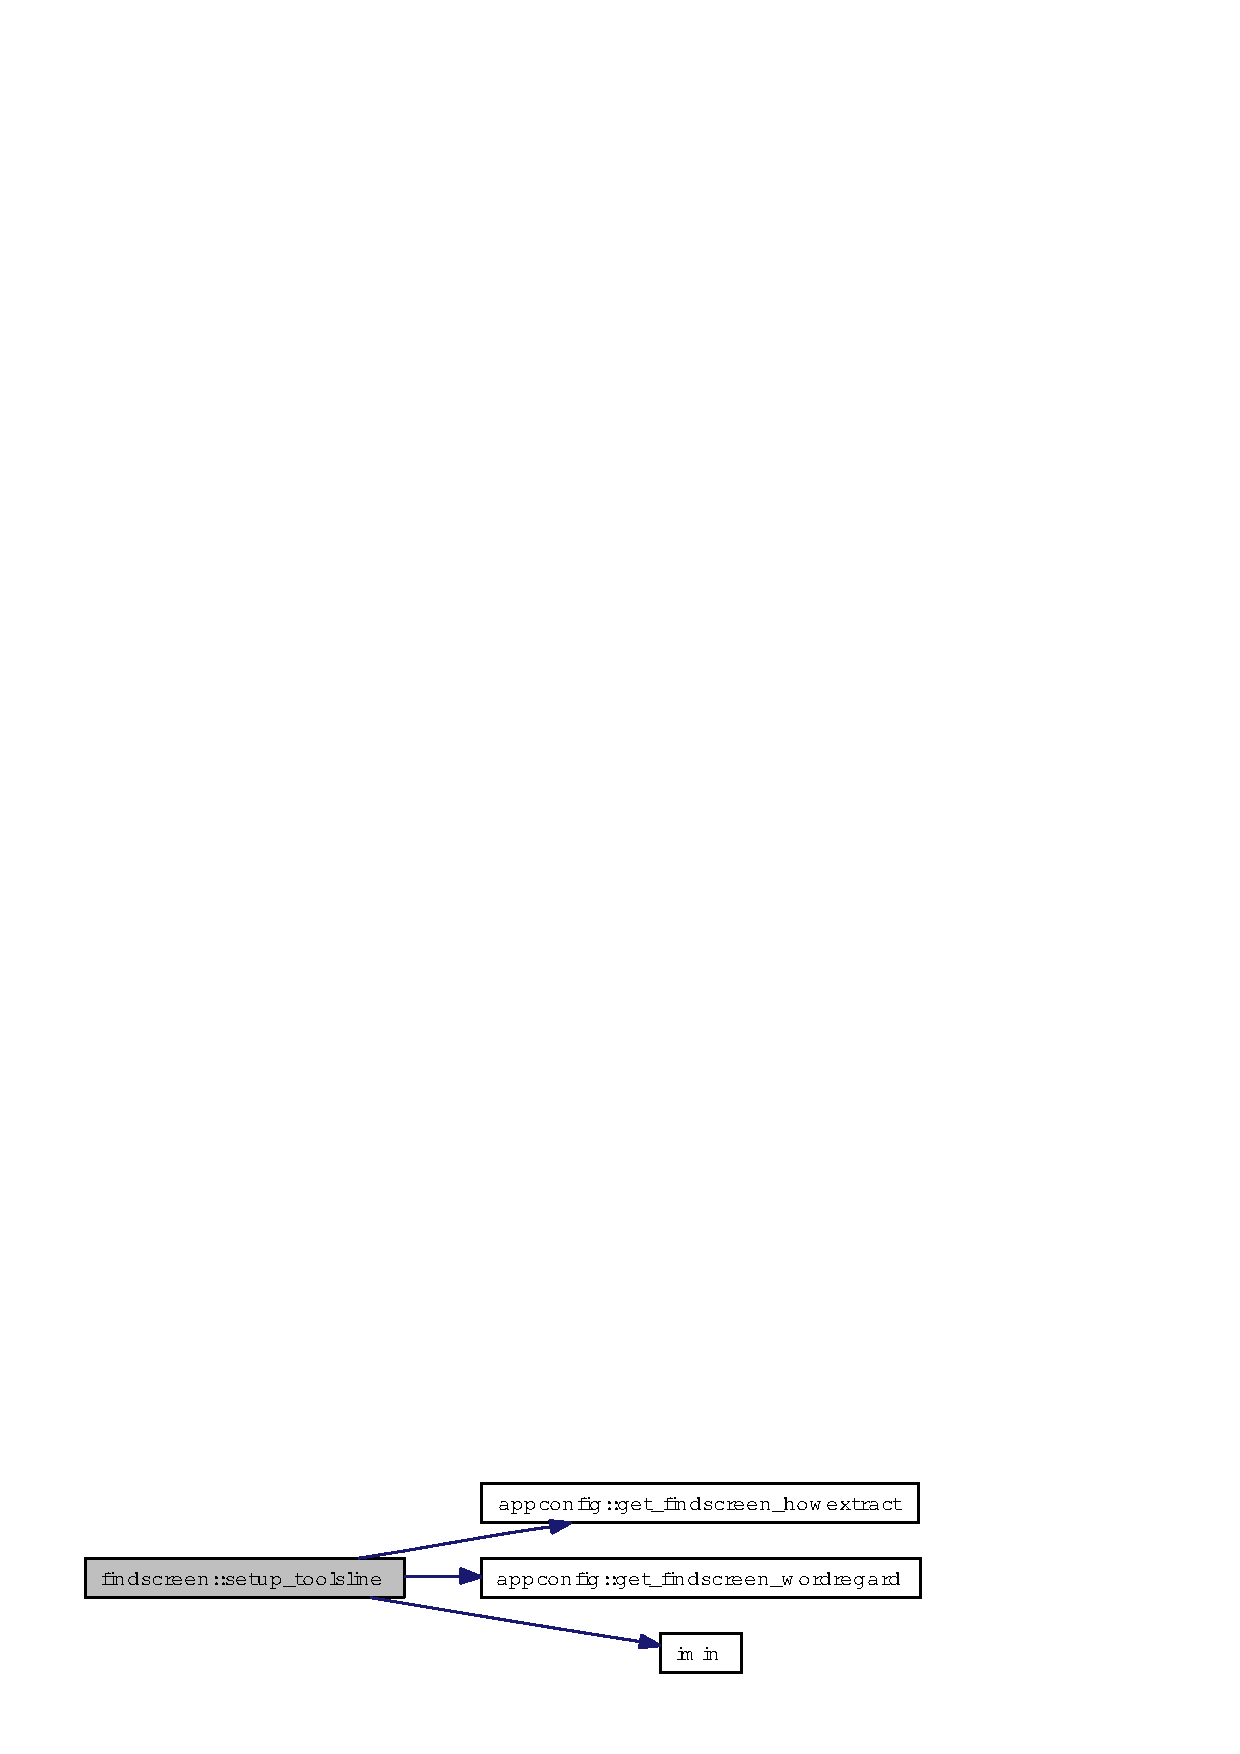
\includegraphics[width=223pt]{classfindscreen_21d3d00b4559ddbafc3cf6332a422a16_cgraph}
\end{center}
\end{figure}


Here is the caller graph for this function:\begin{figure}[H]
\begin{center}
\leavevmode
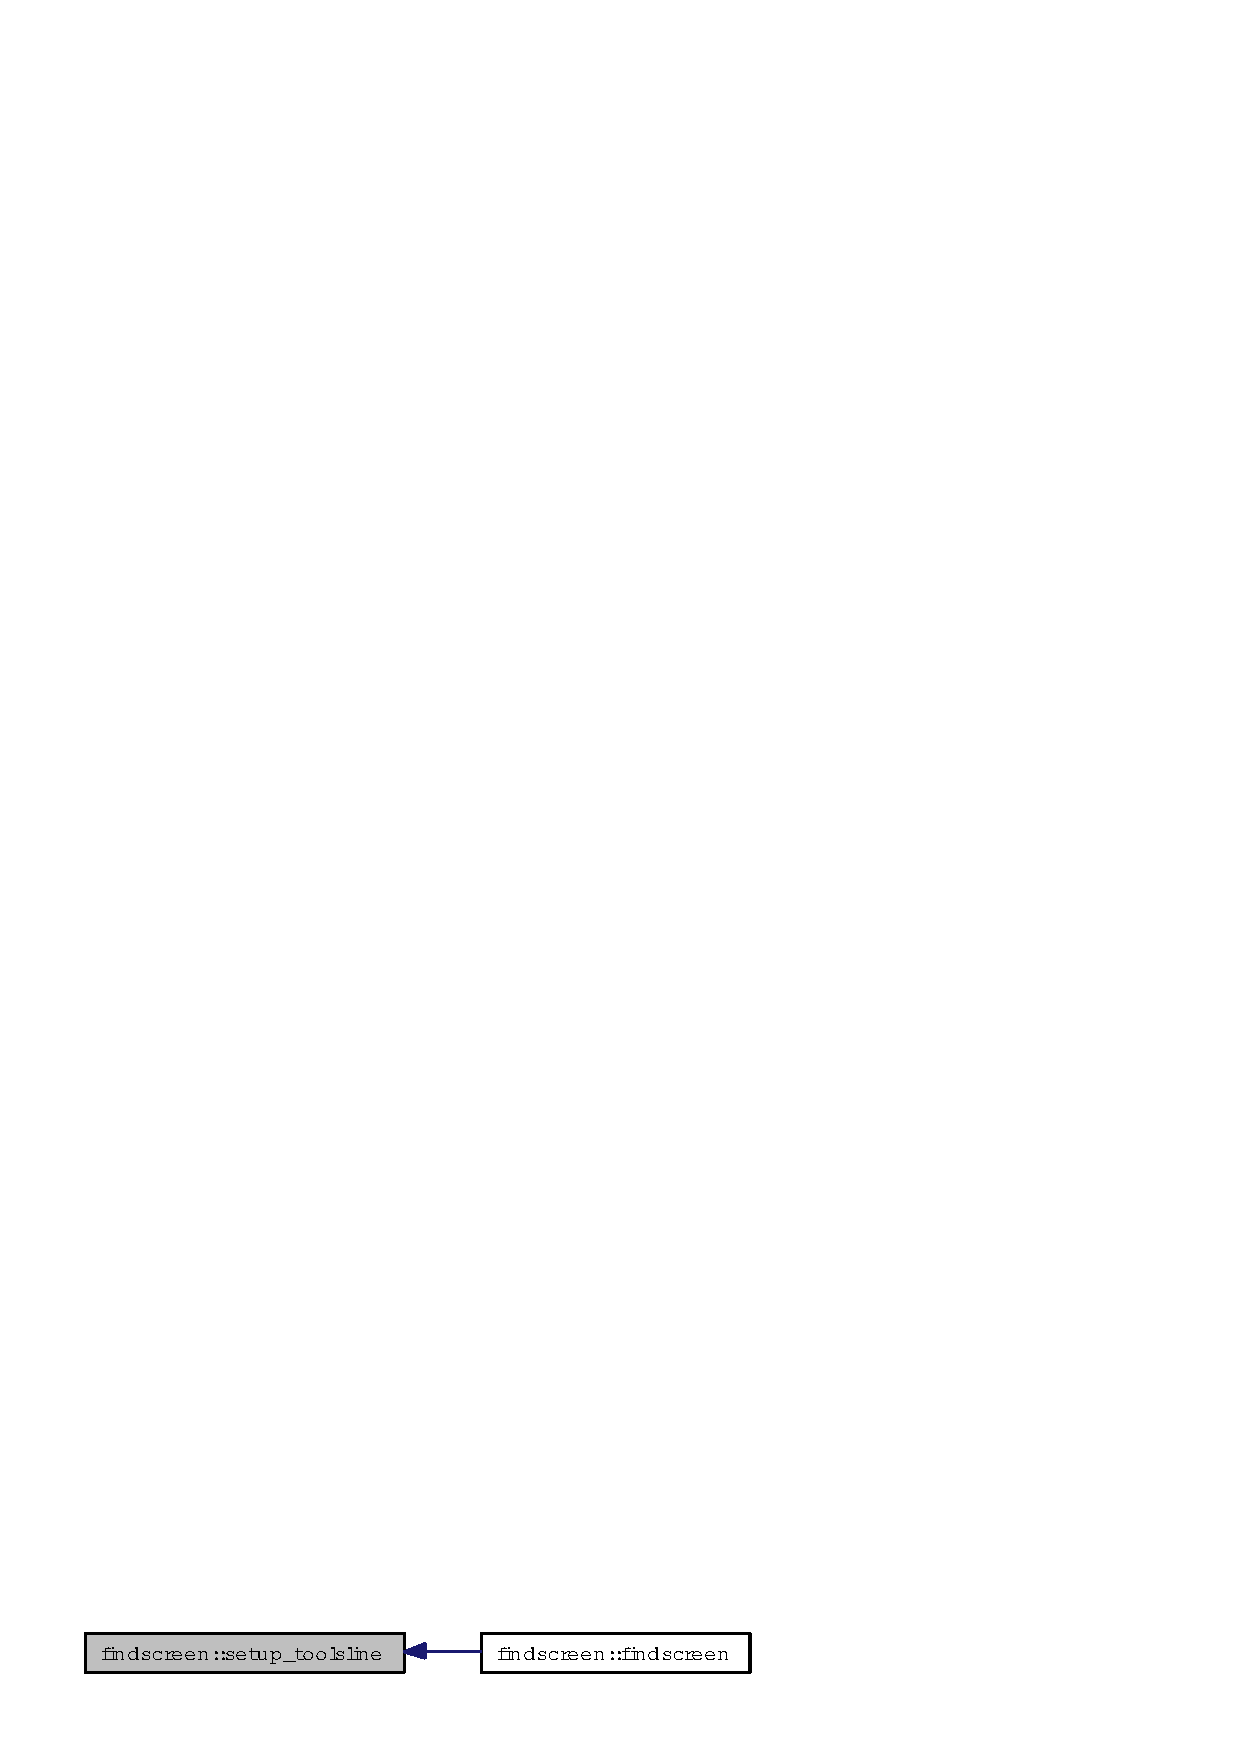
\includegraphics[width=182pt]{classfindscreen_21d3d00b4559ddbafc3cf6332a422a16_icgraph}
\end{center}
\end{figure}
\index{findscreen@{findscreen}!assembly_toolsline@{assembly\_\-toolsline}}
\index{assembly_toolsline@{assembly\_\-toolsline}!findscreen@{findscreen}}
\subsubsection{\setlength{\rightskip}{0pt plus 5cm}void findscreen::assembly\_\-toolsline (void)\hspace{0.3cm}{\tt  [private]}}\label{classfindscreen_88fd4b839652ca0b18ad6e9c270d1c61}




Definition at line 74 of file findscreen.cpp.

References closebutton, findstart, findtext, howextract, placeupclosebutton, toolsline, and wordregard.

Referenced by findscreen().

Here is the caller graph for this function:\begin{figure}[H]
\begin{center}
\leavevmode
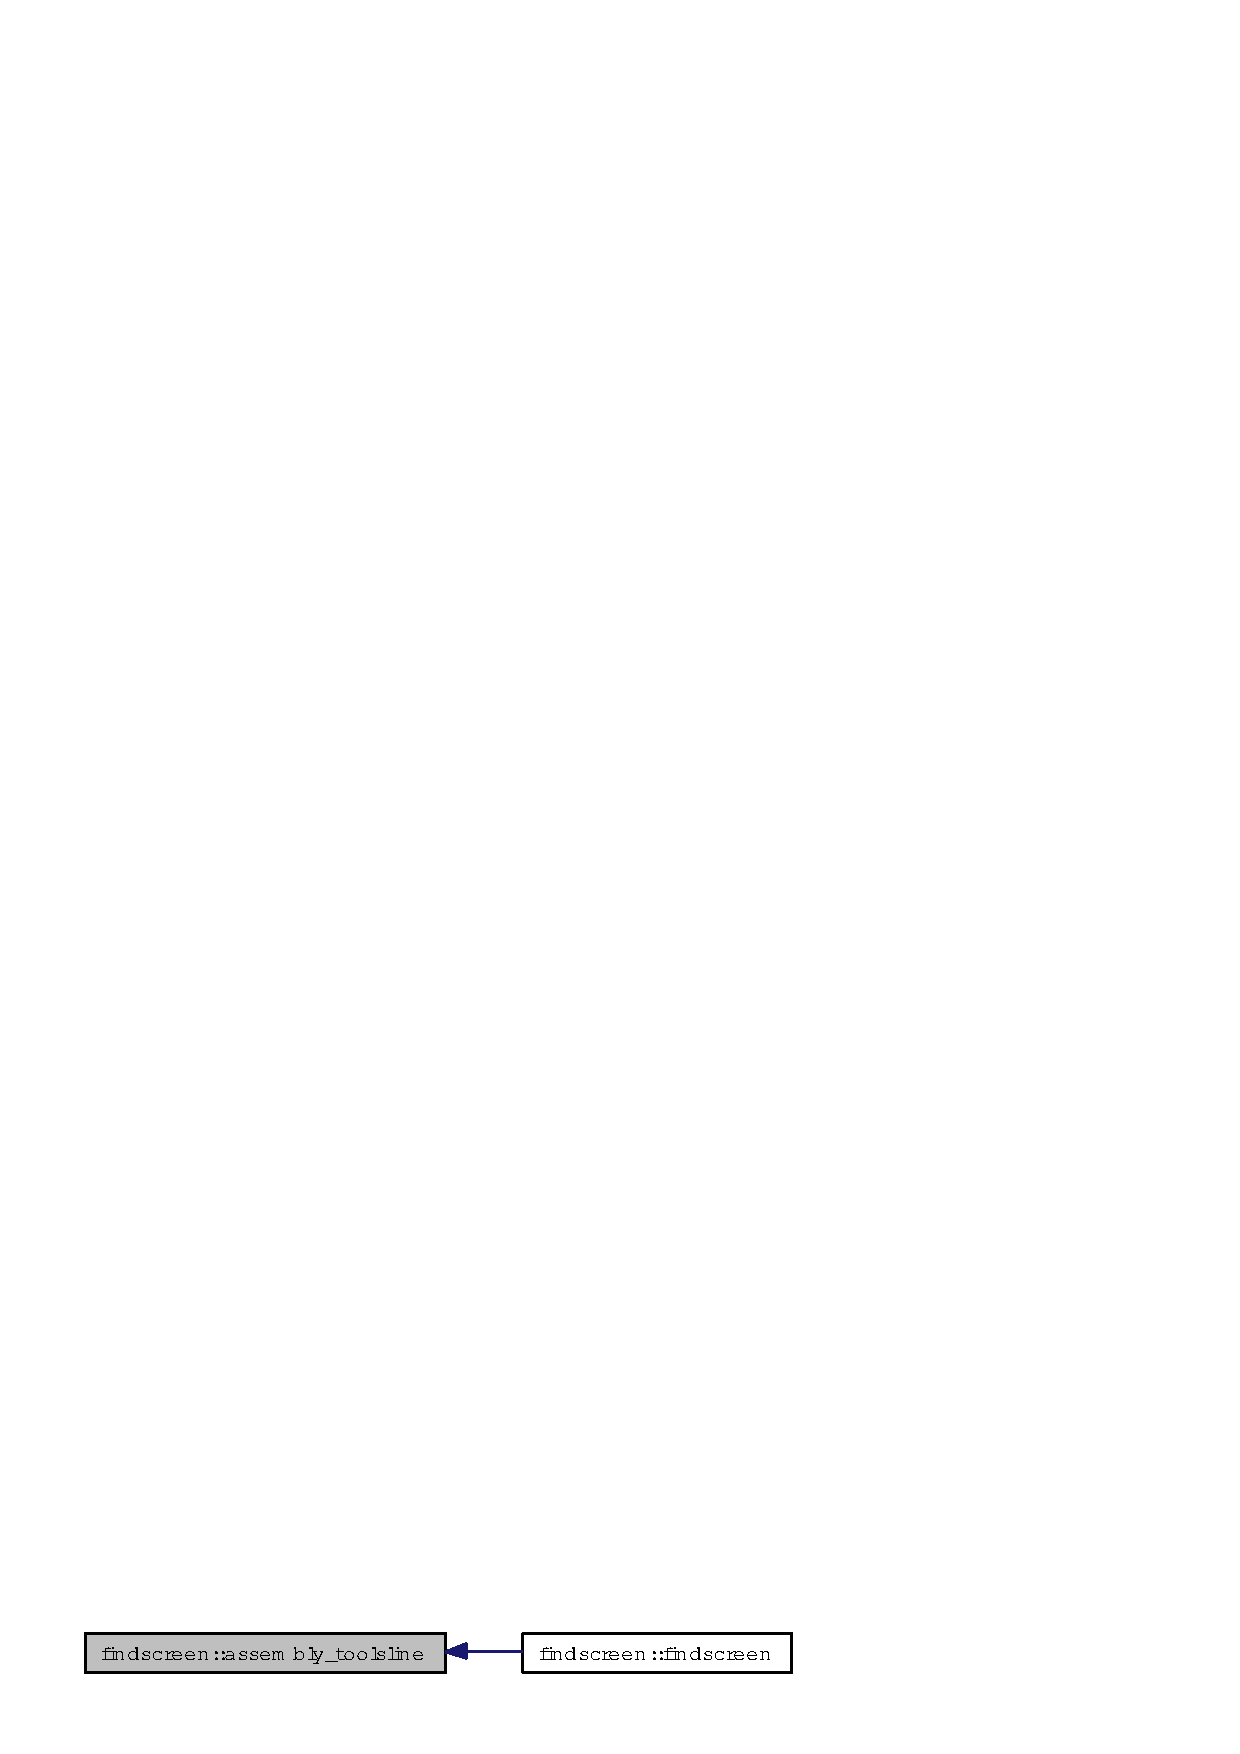
\includegraphics[width=192pt]{classfindscreen_88fd4b839652ca0b18ad6e9c270d1c61_icgraph}
\end{center}
\end{figure}
\index{findscreen@{findscreen}!setup_wherefindline@{setup\_\-wherefindline}}
\index{setup_wherefindline@{setup\_\-wherefindline}!findscreen@{findscreen}}
\subsubsection{\setlength{\rightskip}{0pt plus 5cm}void findscreen::setup\_\-wherefindline (void)\hspace{0.3cm}{\tt  [private]}}\label{classfindscreen_2adcd1d1239878bd53219355a809308c}




Definition at line 97 of file findscreen.cpp.

References find\_\-in\_\-author, find\_\-in\_\-name, find\_\-in\_\-tags, find\_\-in\_\-text, find\_\-in\_\-url, appconfig::get\_\-findscreen\_\-find\_\-in\_\-field(), mytetraconfig, and wherefindlabel.

Referenced by findscreen().

Here is the call graph for this function:\begin{figure}[H]
\begin{center}
\leavevmode
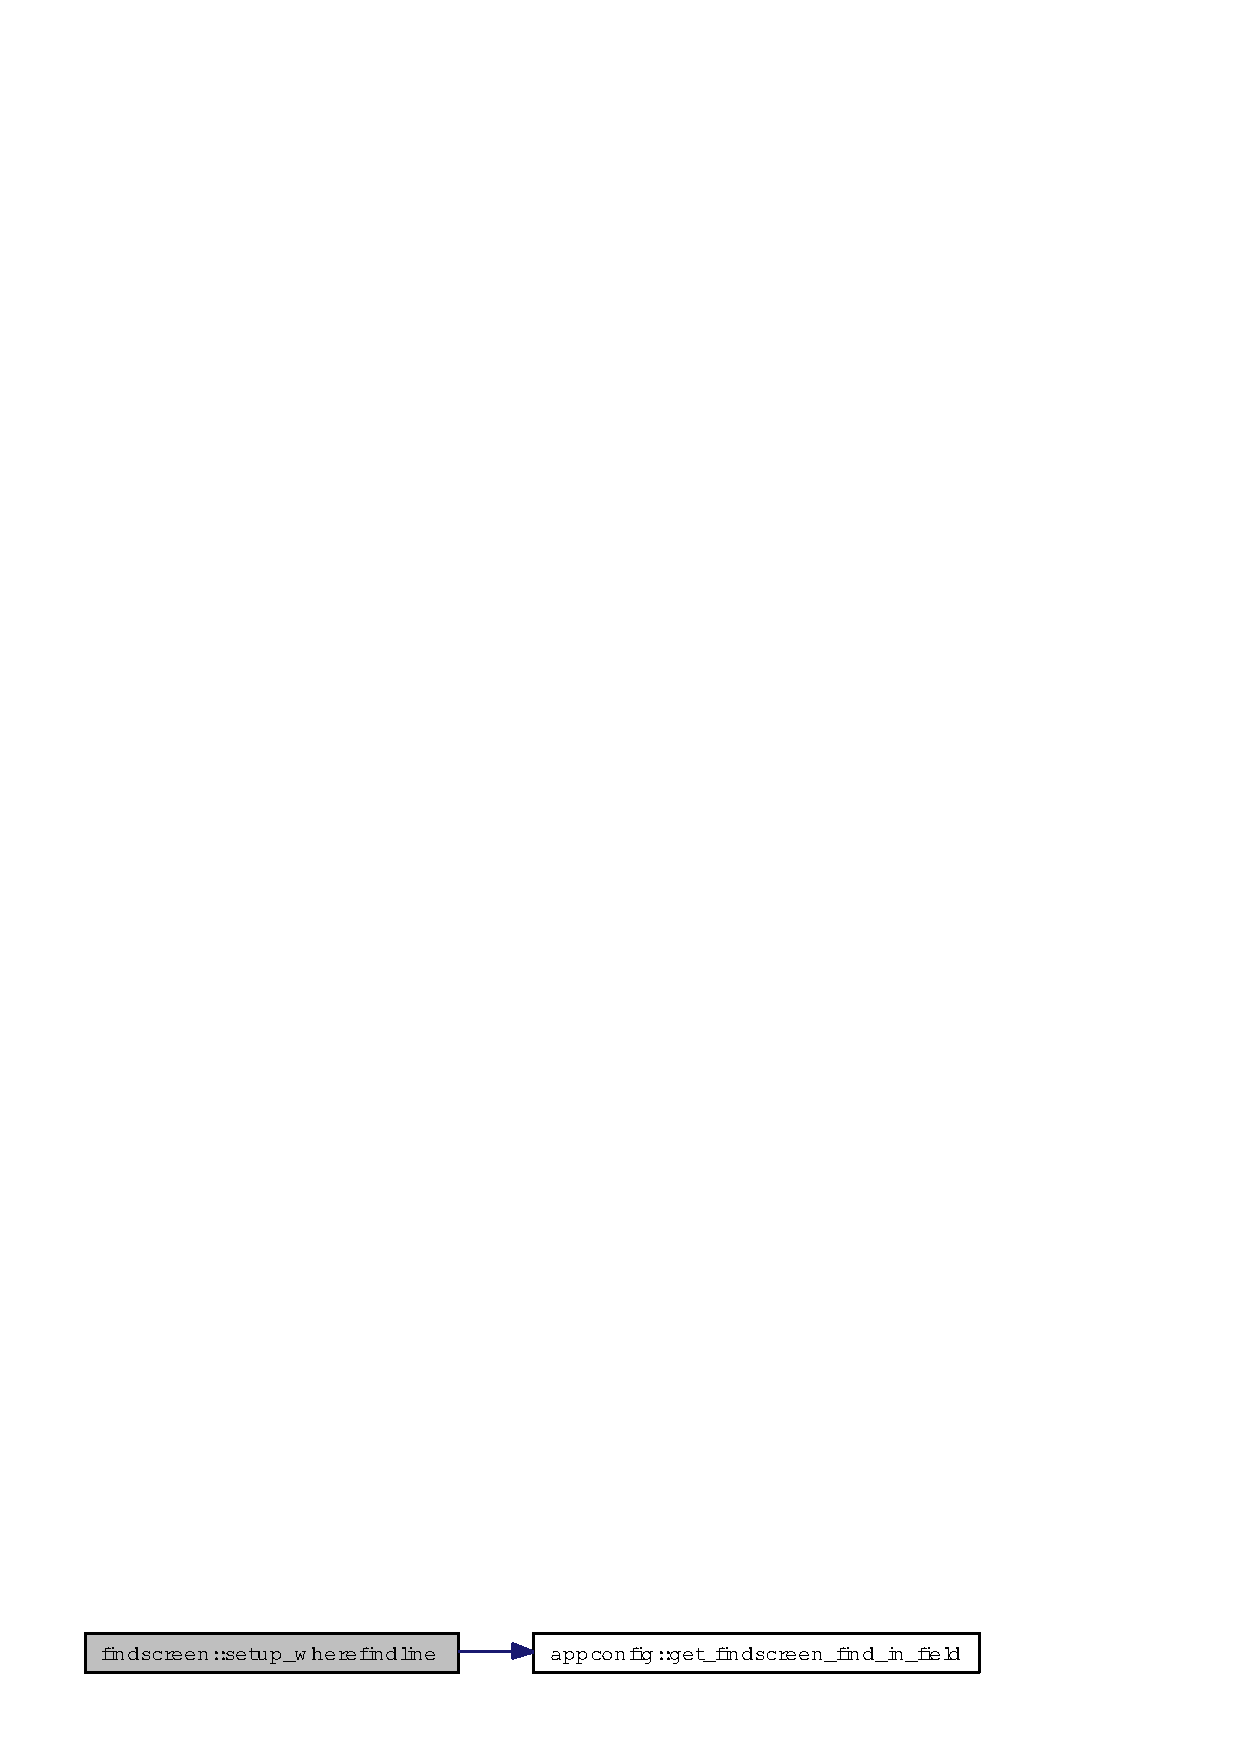
\includegraphics[width=237pt]{classfindscreen_2adcd1d1239878bd53219355a809308c_cgraph}
\end{center}
\end{figure}


Here is the caller graph for this function:\begin{figure}[H]
\begin{center}
\leavevmode
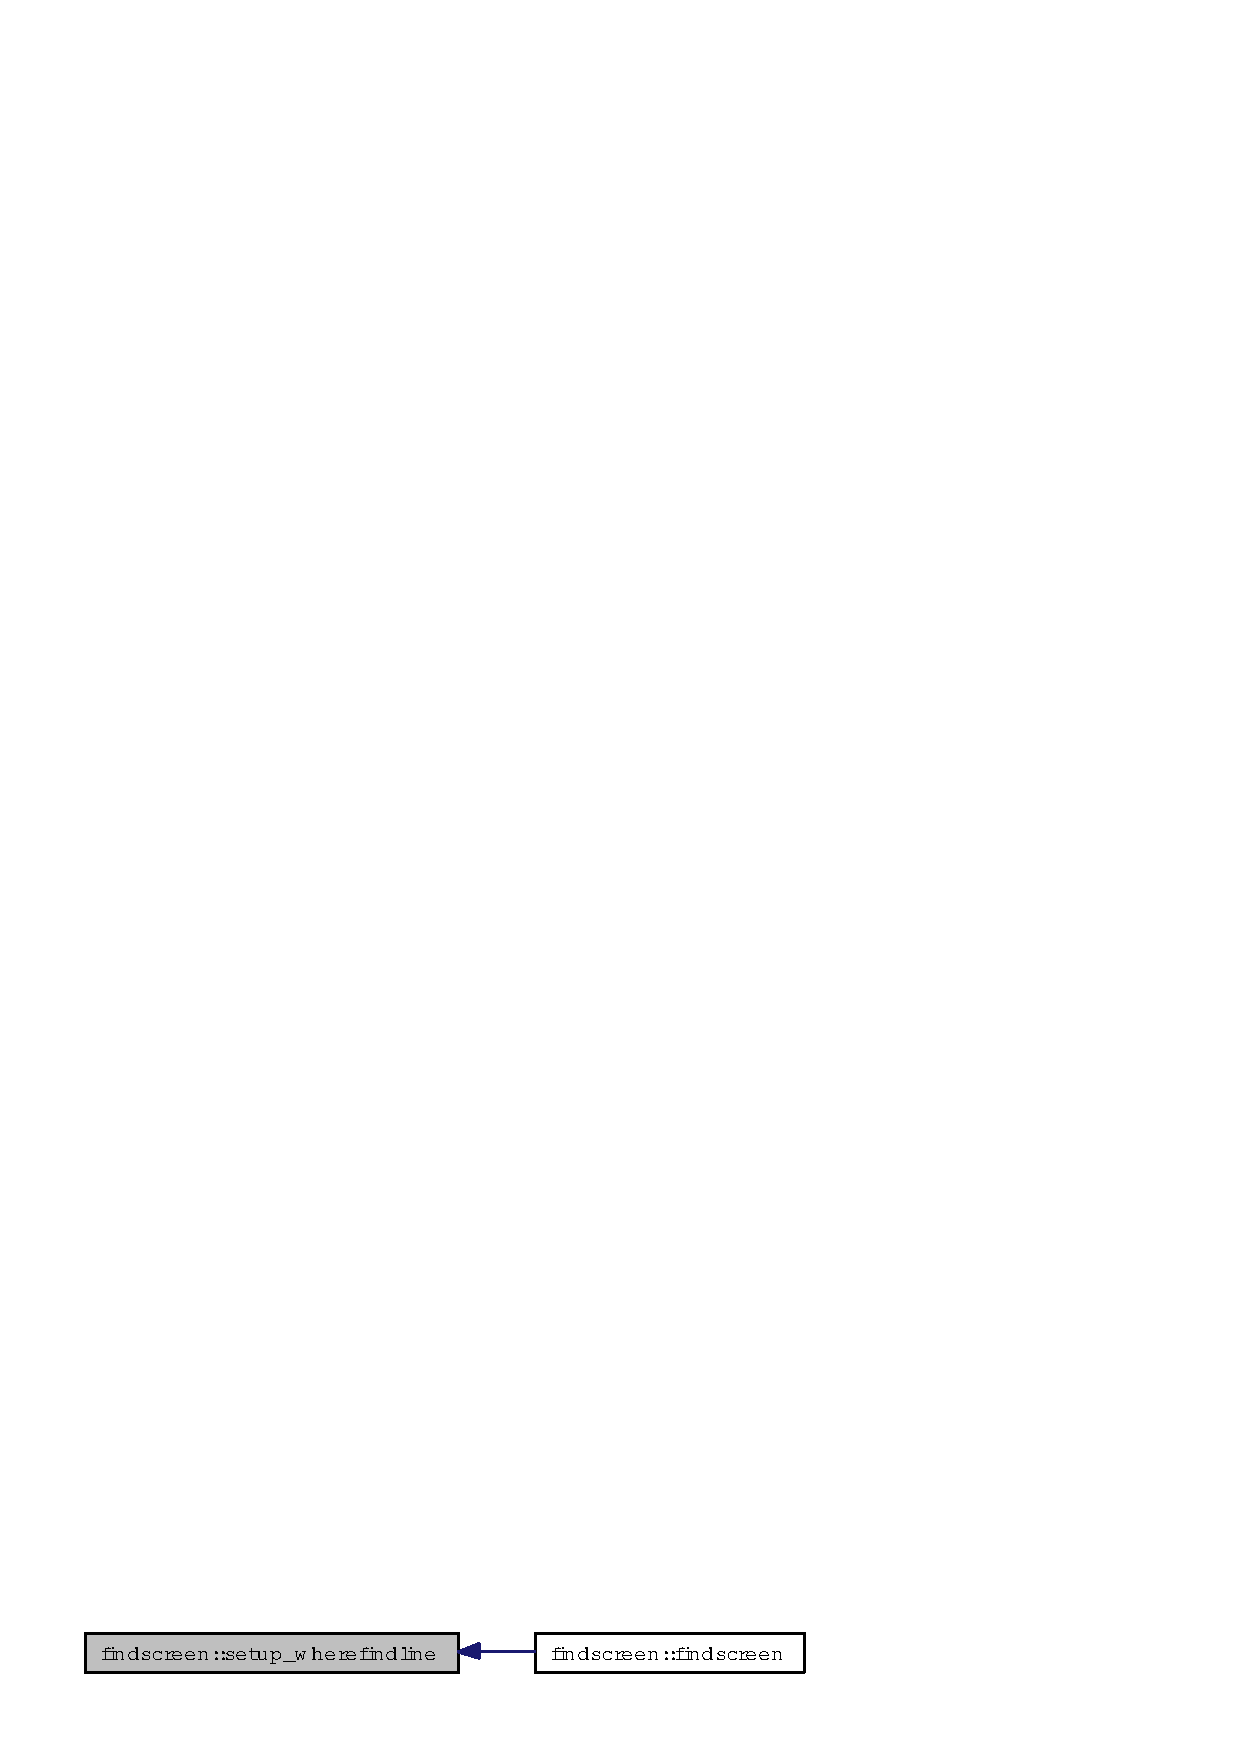
\includegraphics[width=195pt]{classfindscreen_2adcd1d1239878bd53219355a809308c_icgraph}
\end{center}
\end{figure}
\index{findscreen@{findscreen}!assembly_wherefindline@{assembly\_\-wherefindline}}
\index{assembly_wherefindline@{assembly\_\-wherefindline}!findscreen@{findscreen}}
\subsubsection{\setlength{\rightskip}{0pt plus 5cm}void findscreen::assembly\_\-wherefindline (void)\hspace{0.3cm}{\tt  [private]}}\label{classfindscreen_69dc9172d0b787b30bf9793412c65303}




Definition at line 118 of file findscreen.cpp.

References find\_\-in\_\-author, find\_\-in\_\-name, find\_\-in\_\-tags, find\_\-in\_\-text, find\_\-in\_\-url, wherefindlabel, and wherefindline.

Referenced by findscreen().

Here is the caller graph for this function:\begin{figure}[H]
\begin{center}
\leavevmode
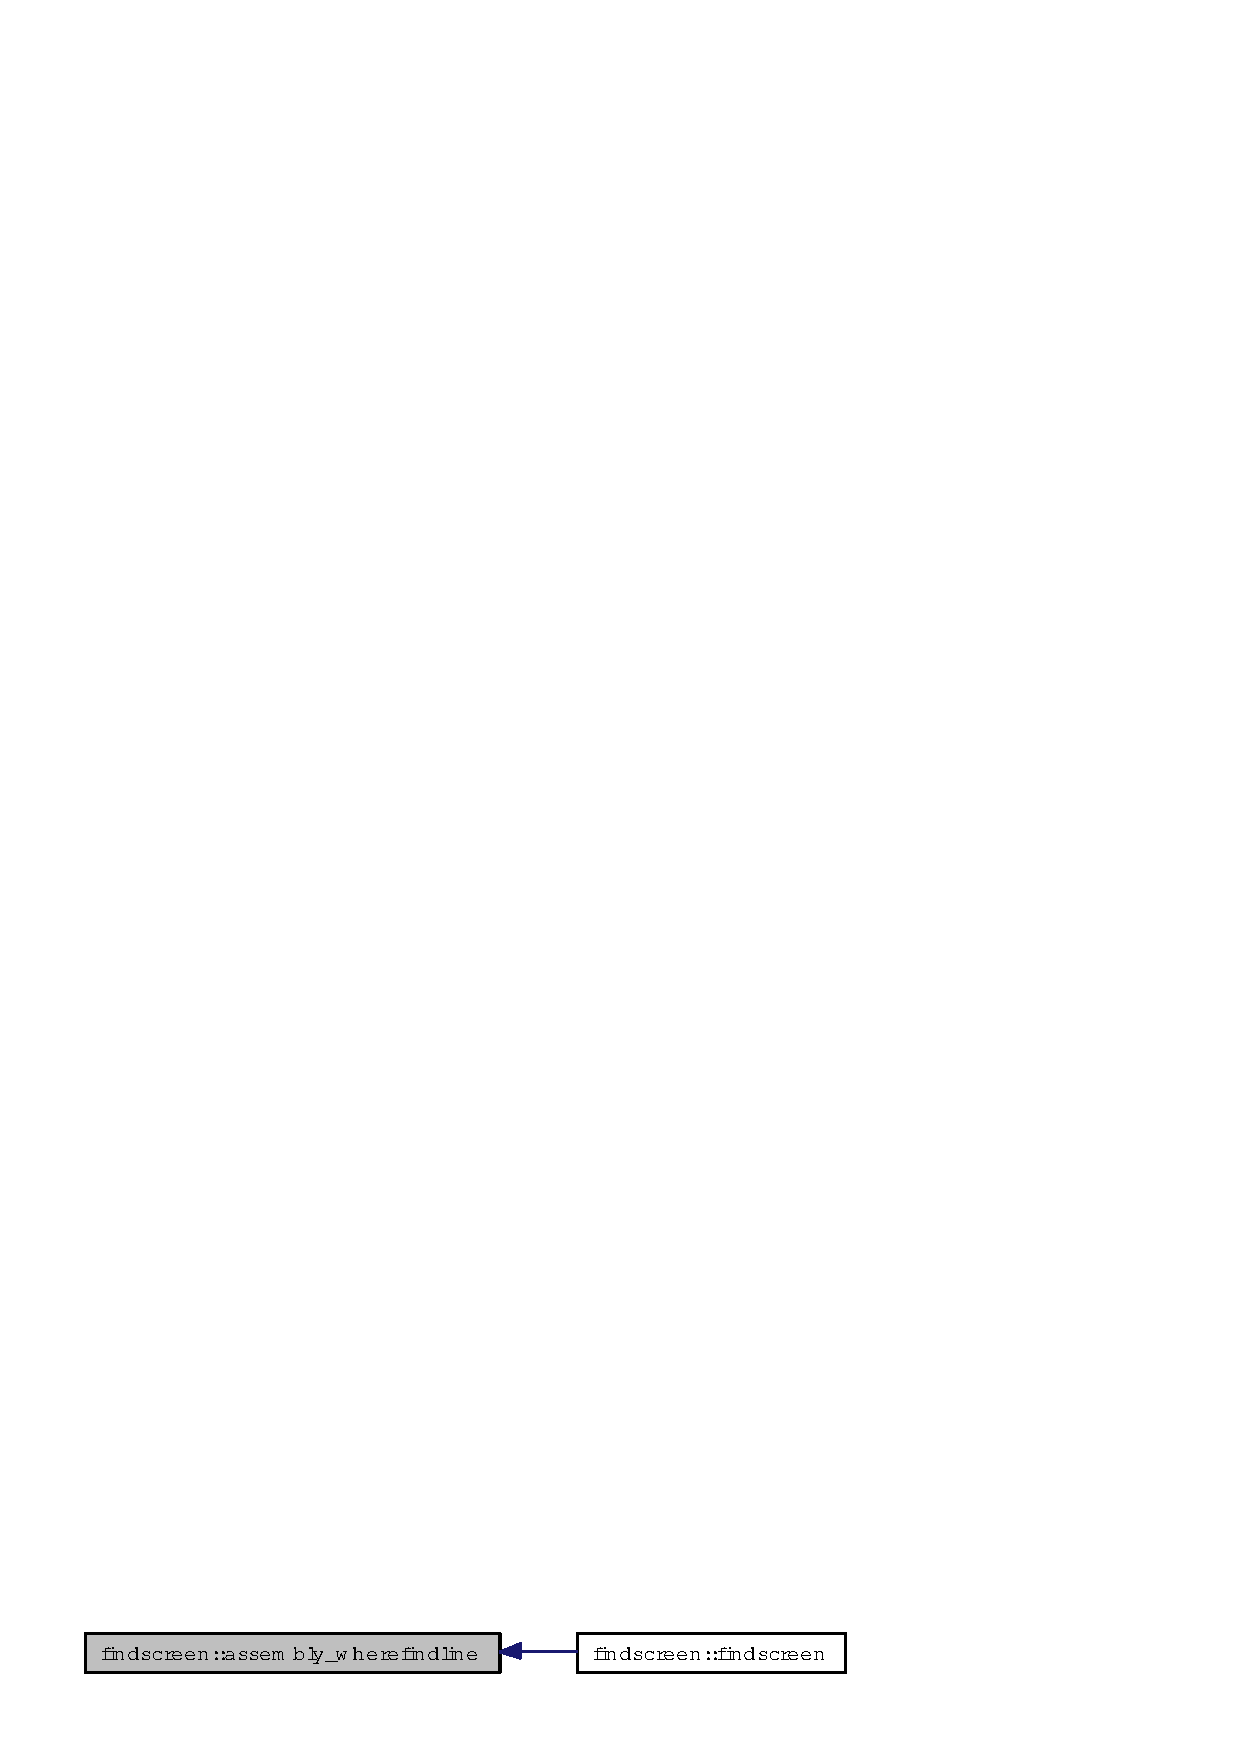
\includegraphics[width=205pt]{classfindscreen_69dc9172d0b787b30bf9793412c65303_icgraph}
\end{center}
\end{figure}
\index{findscreen@{findscreen}!setup_ui@{setup\_\-ui}}
\index{setup_ui@{setup\_\-ui}!findscreen@{findscreen}}
\subsubsection{\setlength{\rightskip}{0pt plus 5cm}void findscreen::setup\_\-ui (void)\hspace{0.3cm}{\tt  [private]}}\label{classfindscreen_b8d98fa703f0a8eb08a77b197b2a0d4f}




Definition at line 177 of file findscreen.cpp.

References findtable.

Referenced by findscreen().

Here is the caller graph for this function:\begin{figure}[H]
\begin{center}
\leavevmode
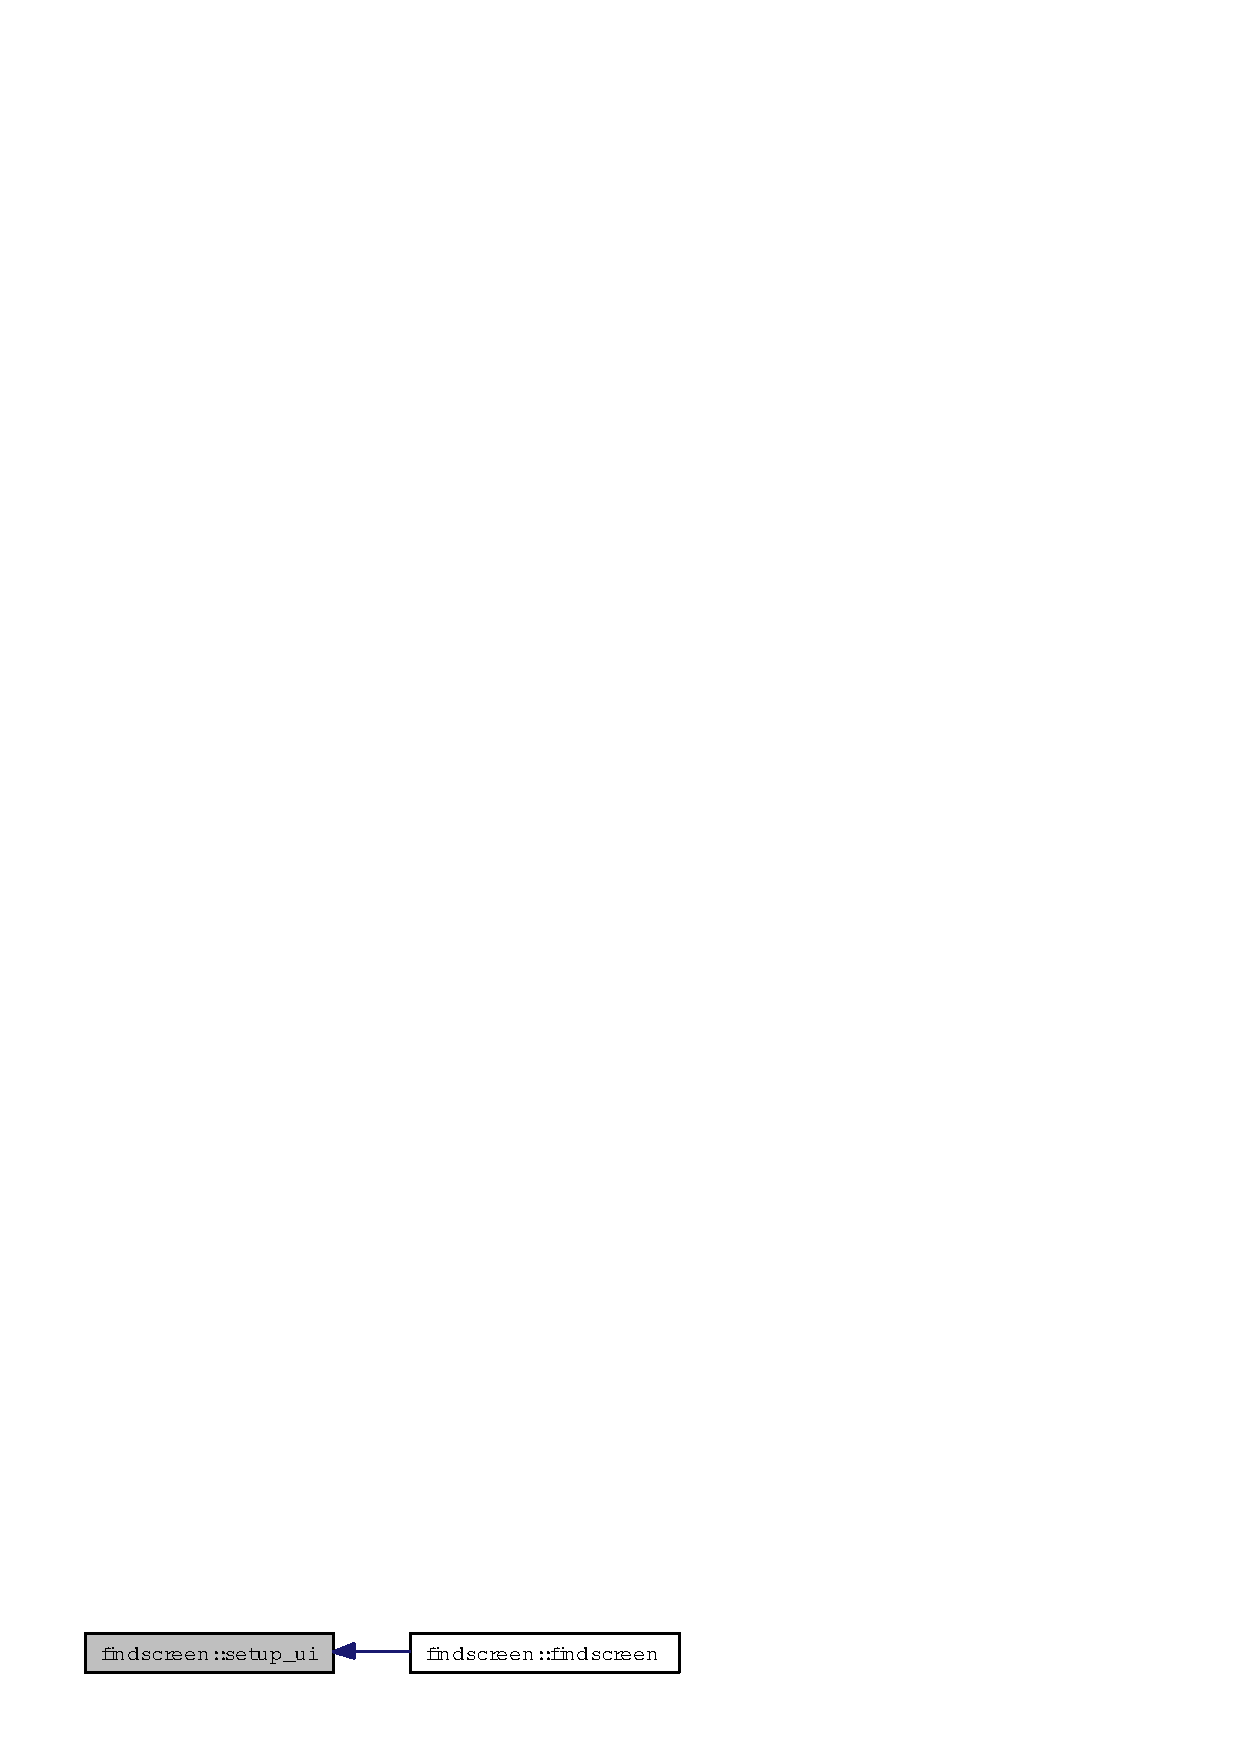
\includegraphics[width=165pt]{classfindscreen_b8d98fa703f0a8eb08a77b197b2a0d4f_icgraph}
\end{center}
\end{figure}
\index{findscreen@{findscreen}!assembly@{assembly}}
\index{assembly@{assembly}!findscreen@{findscreen}}
\subsubsection{\setlength{\rightskip}{0pt plus 5cm}void findscreen::assembly (void)\hspace{0.3cm}{\tt  [private]}}\label{classfindscreen_f8df2e8eb659306b1395d499e2e2595e}




Definition at line 184 of file findscreen.cpp.

References centrallayout, findtable, toolsline, and wherefindline.

Referenced by findscreen().

Here is the caller graph for this function:\begin{figure}[H]
\begin{center}
\leavevmode
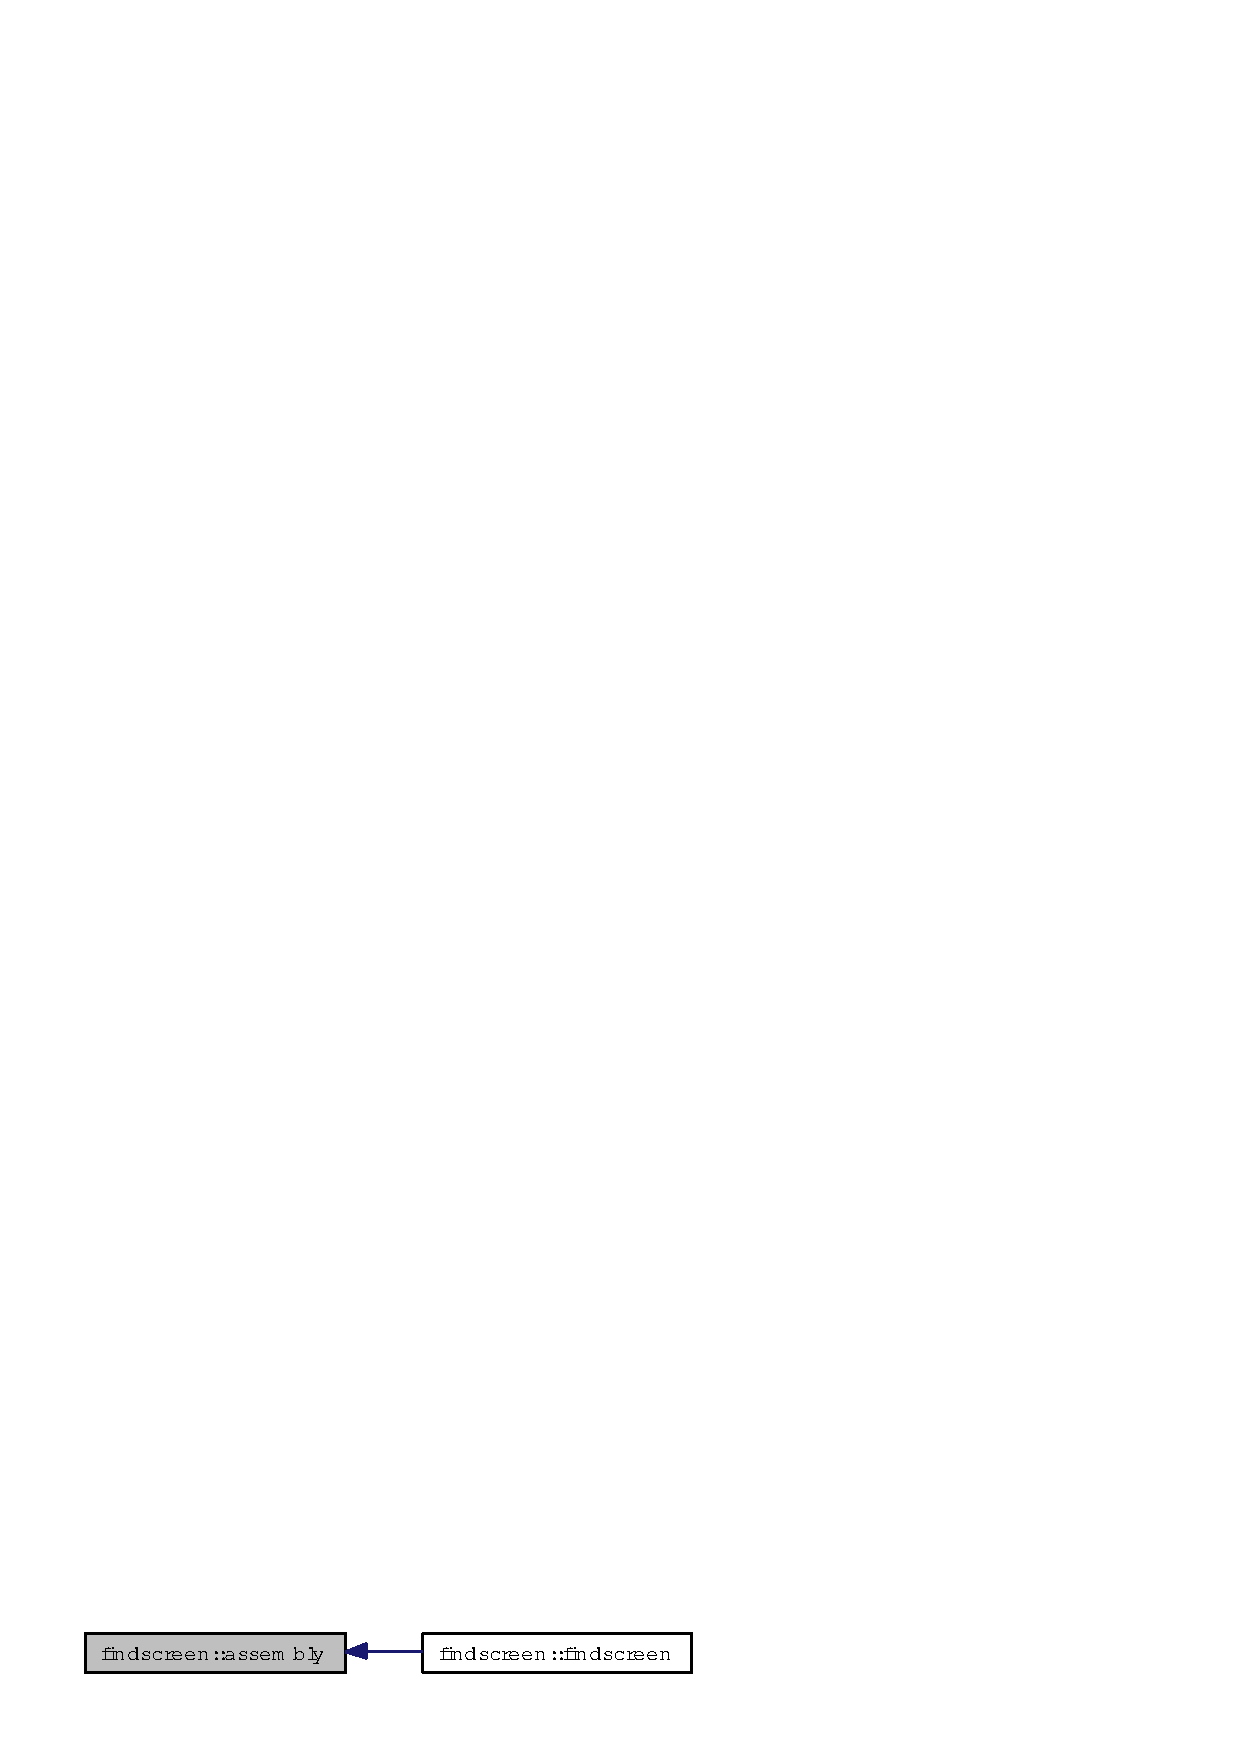
\includegraphics[width=168pt]{classfindscreen_f8df2e8eb659306b1395d499e2e2595e_icgraph}
\end{center}
\end{figure}
\index{findscreen@{findscreen}!setup_signals@{setup\_\-signals}}
\index{setup_signals@{setup\_\-signals}!findscreen@{findscreen}}
\subsubsection{\setlength{\rightskip}{0pt plus 5cm}void findscreen::setup\_\-signals (void)\hspace{0.3cm}{\tt  [private]}}\label{classfindscreen_0dfe30d416c78957e826e6ba6ad6e865}




Definition at line 135 of file findscreen.cpp.

References changed\_\-find\_\-in\_\-author(), changed\_\-find\_\-in\_\-name(), changed\_\-find\_\-in\_\-tags(), changed\_\-find\_\-in\_\-text(), changed\_\-find\_\-in\_\-url(), changed\_\-howextract(), changed\_\-wordregard(), closebutton, enable\_\-find\_\-button(), find\_\-clicked(), find\_\-in\_\-author, find\_\-in\_\-name, find\_\-in\_\-tags, find\_\-in\_\-text, find\_\-in\_\-url, findstart, findtext, howextract, widget\_\-hide(), and wordregard.

Referenced by findscreen().

Here is the caller graph for this function:\begin{figure}[H]
\begin{center}
\leavevmode
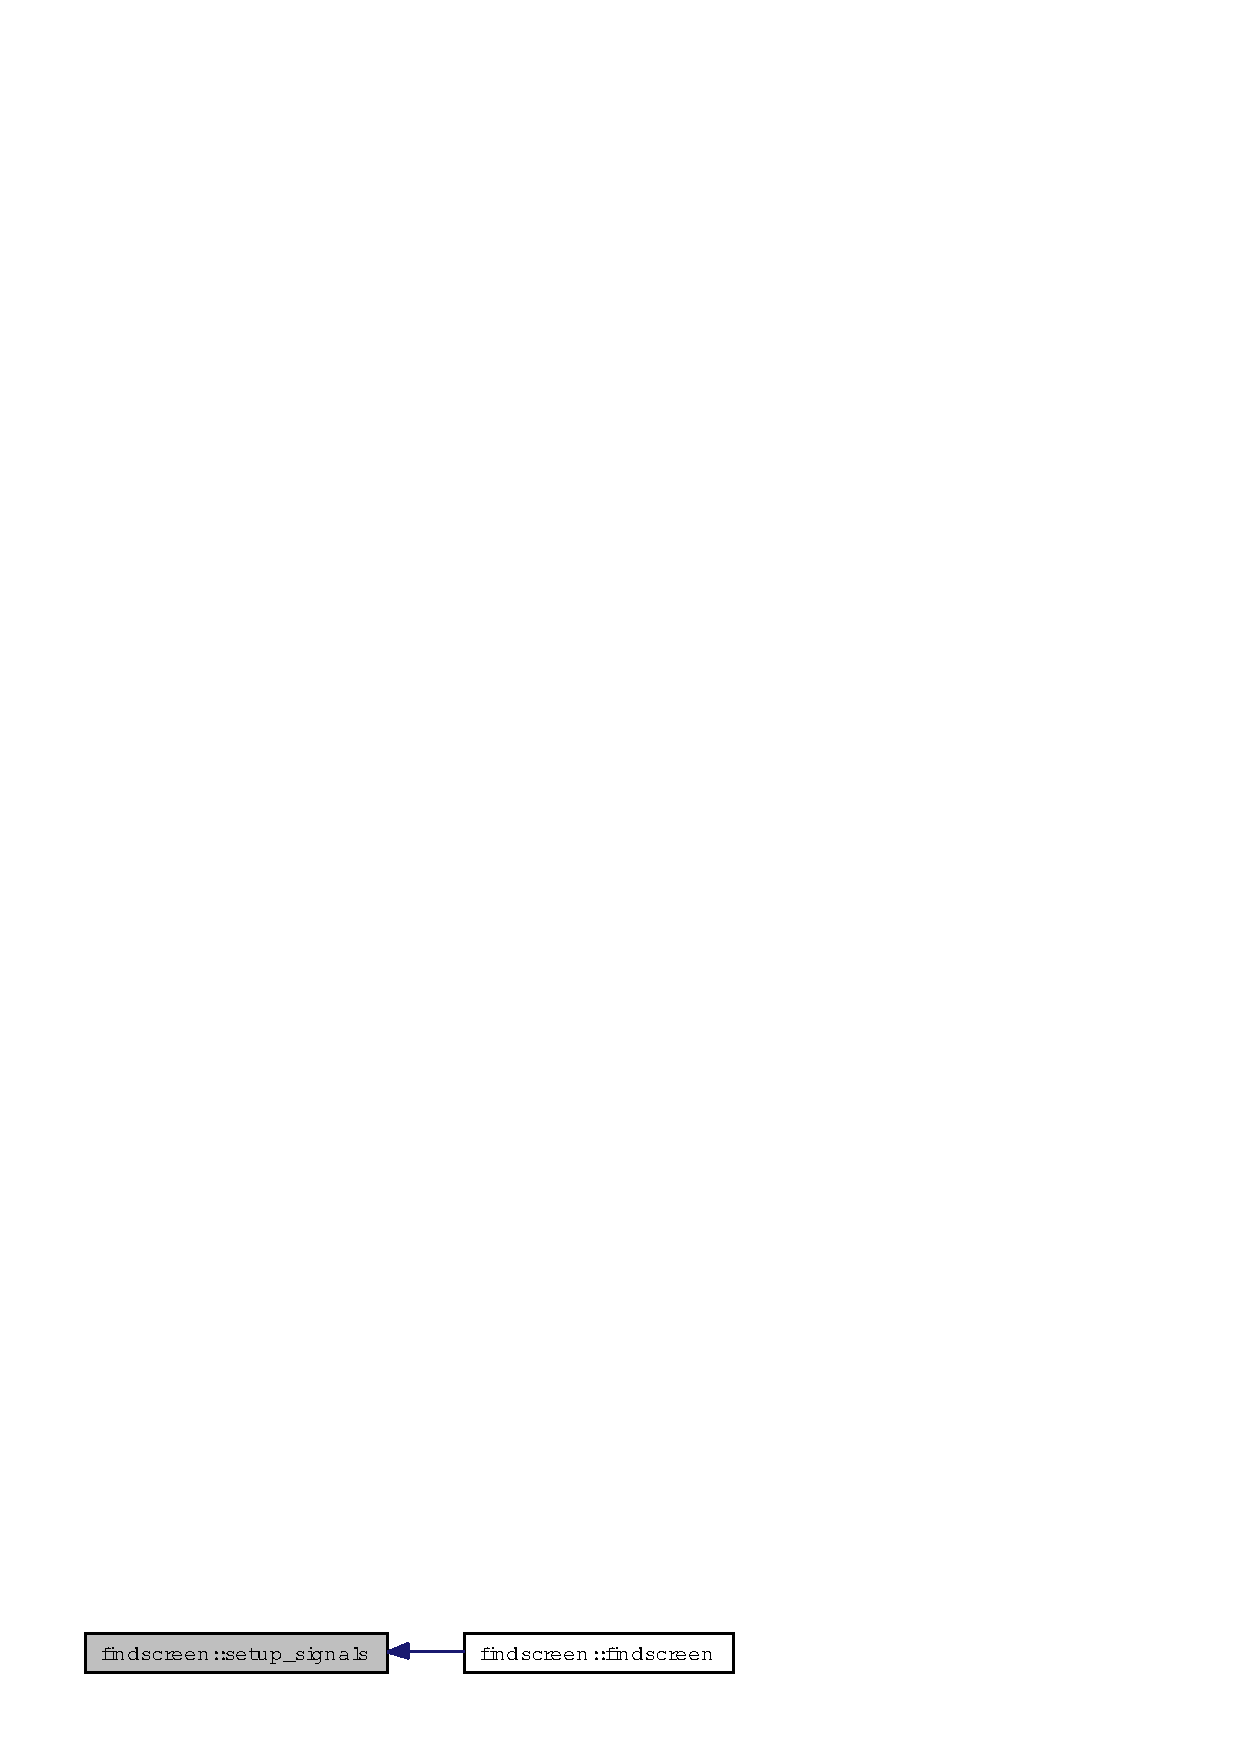
\includegraphics[width=178pt]{classfindscreen_0dfe30d416c78957e826e6ba6ad6e865_icgraph}
\end{center}
\end{figure}
\index{findscreen@{findscreen}!changed_find_in_field@{changed\_\-find\_\-in\_\-field}}
\index{changed_find_in_field@{changed\_\-find\_\-in\_\-field}!findscreen@{findscreen}}
\subsubsection{\setlength{\rightskip}{0pt plus 5cm}void findscreen::changed\_\-find\_\-in\_\-field (QString {\em fieldname}, int {\em state})\hspace{0.3cm}{\tt  [private]}}\label{classfindscreen_dca80696c1d3b77a0ebe8335157bf6e7}




Definition at line 457 of file findscreen.cpp.

References mytetraconfig, and appconfig::set\_\-findscreen\_\-find\_\-in\_\-field().

Referenced by changed\_\-find\_\-in\_\-author(), changed\_\-find\_\-in\_\-name(), changed\_\-find\_\-in\_\-tags(), changed\_\-find\_\-in\_\-text(), and changed\_\-find\_\-in\_\-url().

Here is the call graph for this function:\begin{figure}[H]
\begin{center}
\leavevmode
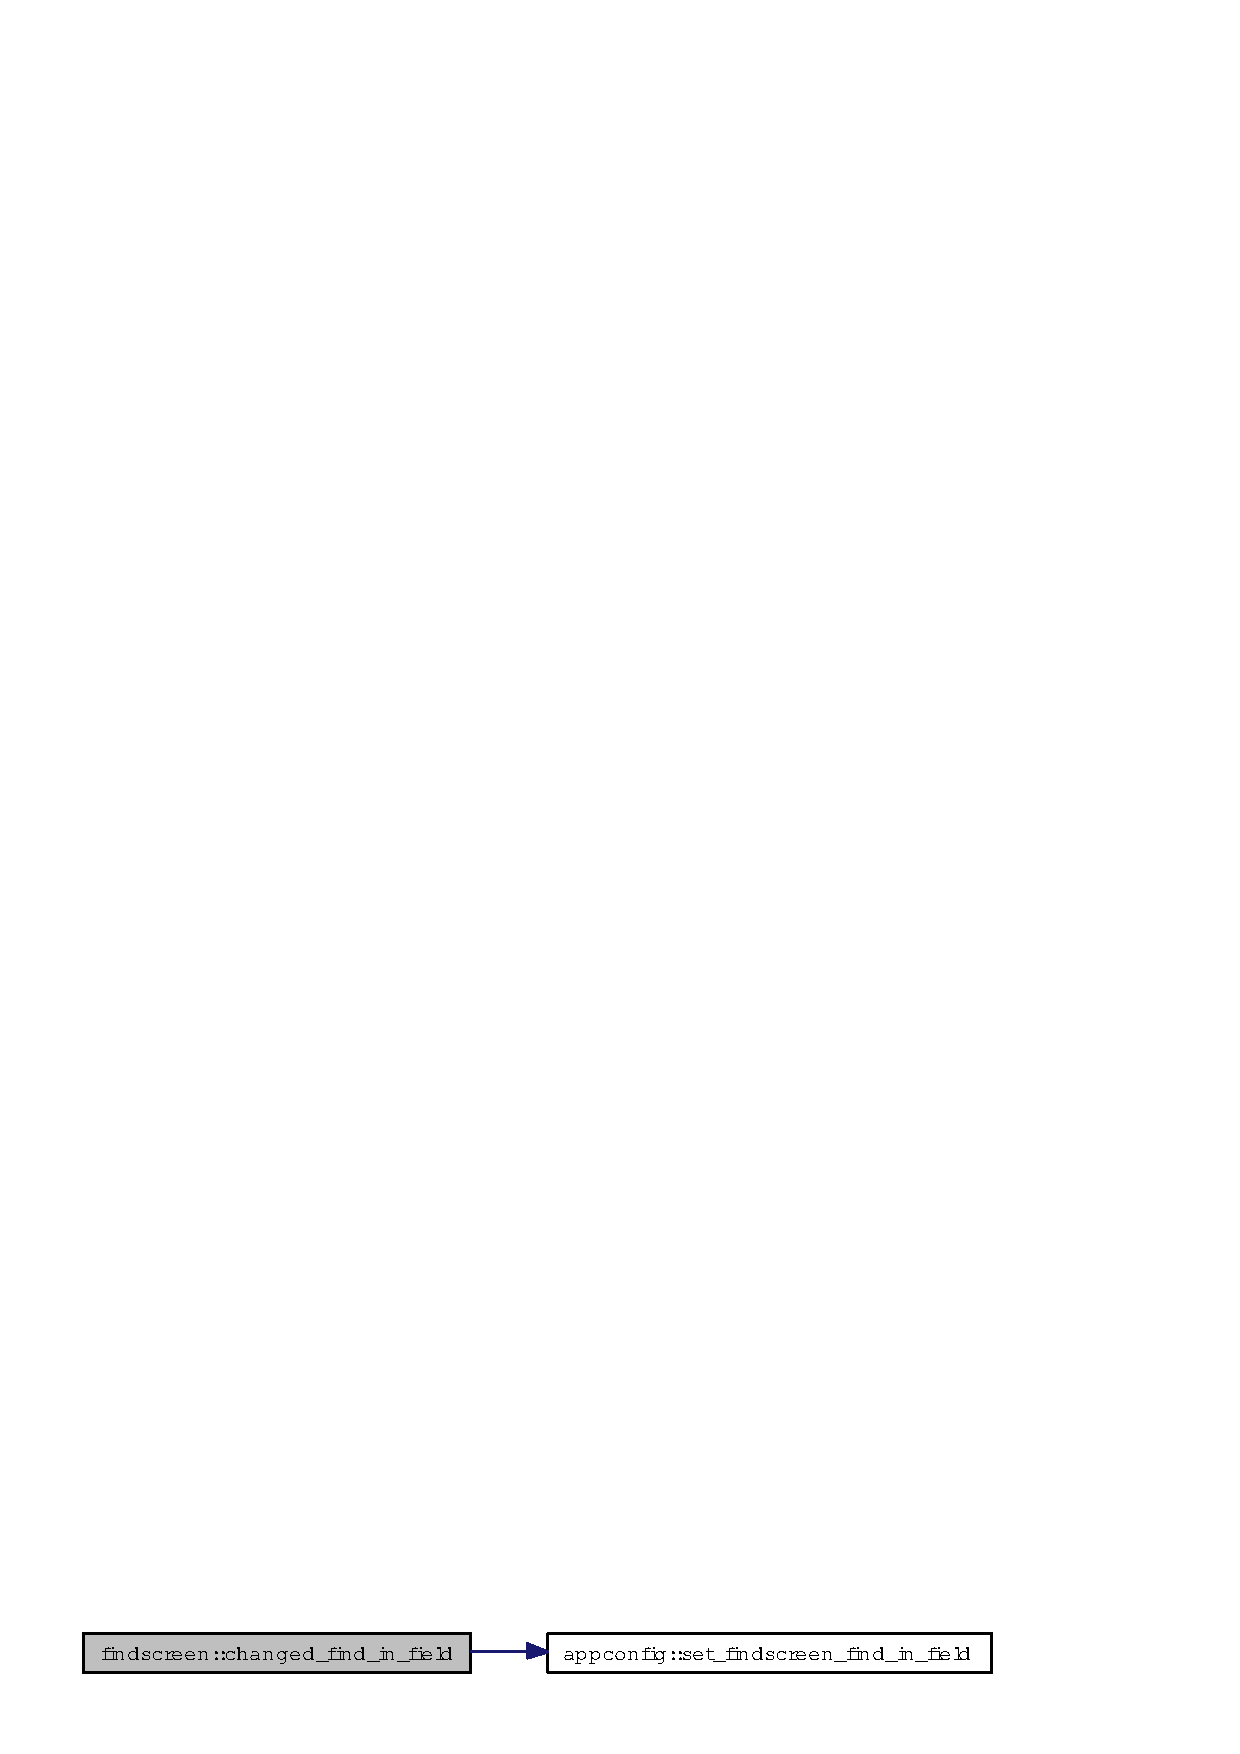
\includegraphics[width=240pt]{classfindscreen_dca80696c1d3b77a0ebe8335157bf6e7_cgraph}
\end{center}
\end{figure}
\index{findscreen@{findscreen}!find_start@{find\_\-start}}
\index{find_start@{find\_\-start}!findscreen@{findscreen}}
\subsubsection{\setlength{\rightskip}{0pt plus 5cm}void findscreen::find\_\-start (void)\hspace{0.3cm}{\tt  [private]}}\label{classfindscreen_c07d8e7cc43f0ea168768e94d7c83099}




Definition at line 263 of file findscreen.cpp.

References findtablewidget::clear\_\-all(), find\_\-recurse(), findtable, Tree\-Model::root\-Item, and findtablewidget::update\_\-columns\_\-width().

Referenced by find\_\-clicked().

Here is the call graph for this function:\begin{figure}[H]
\begin{center}
\leavevmode
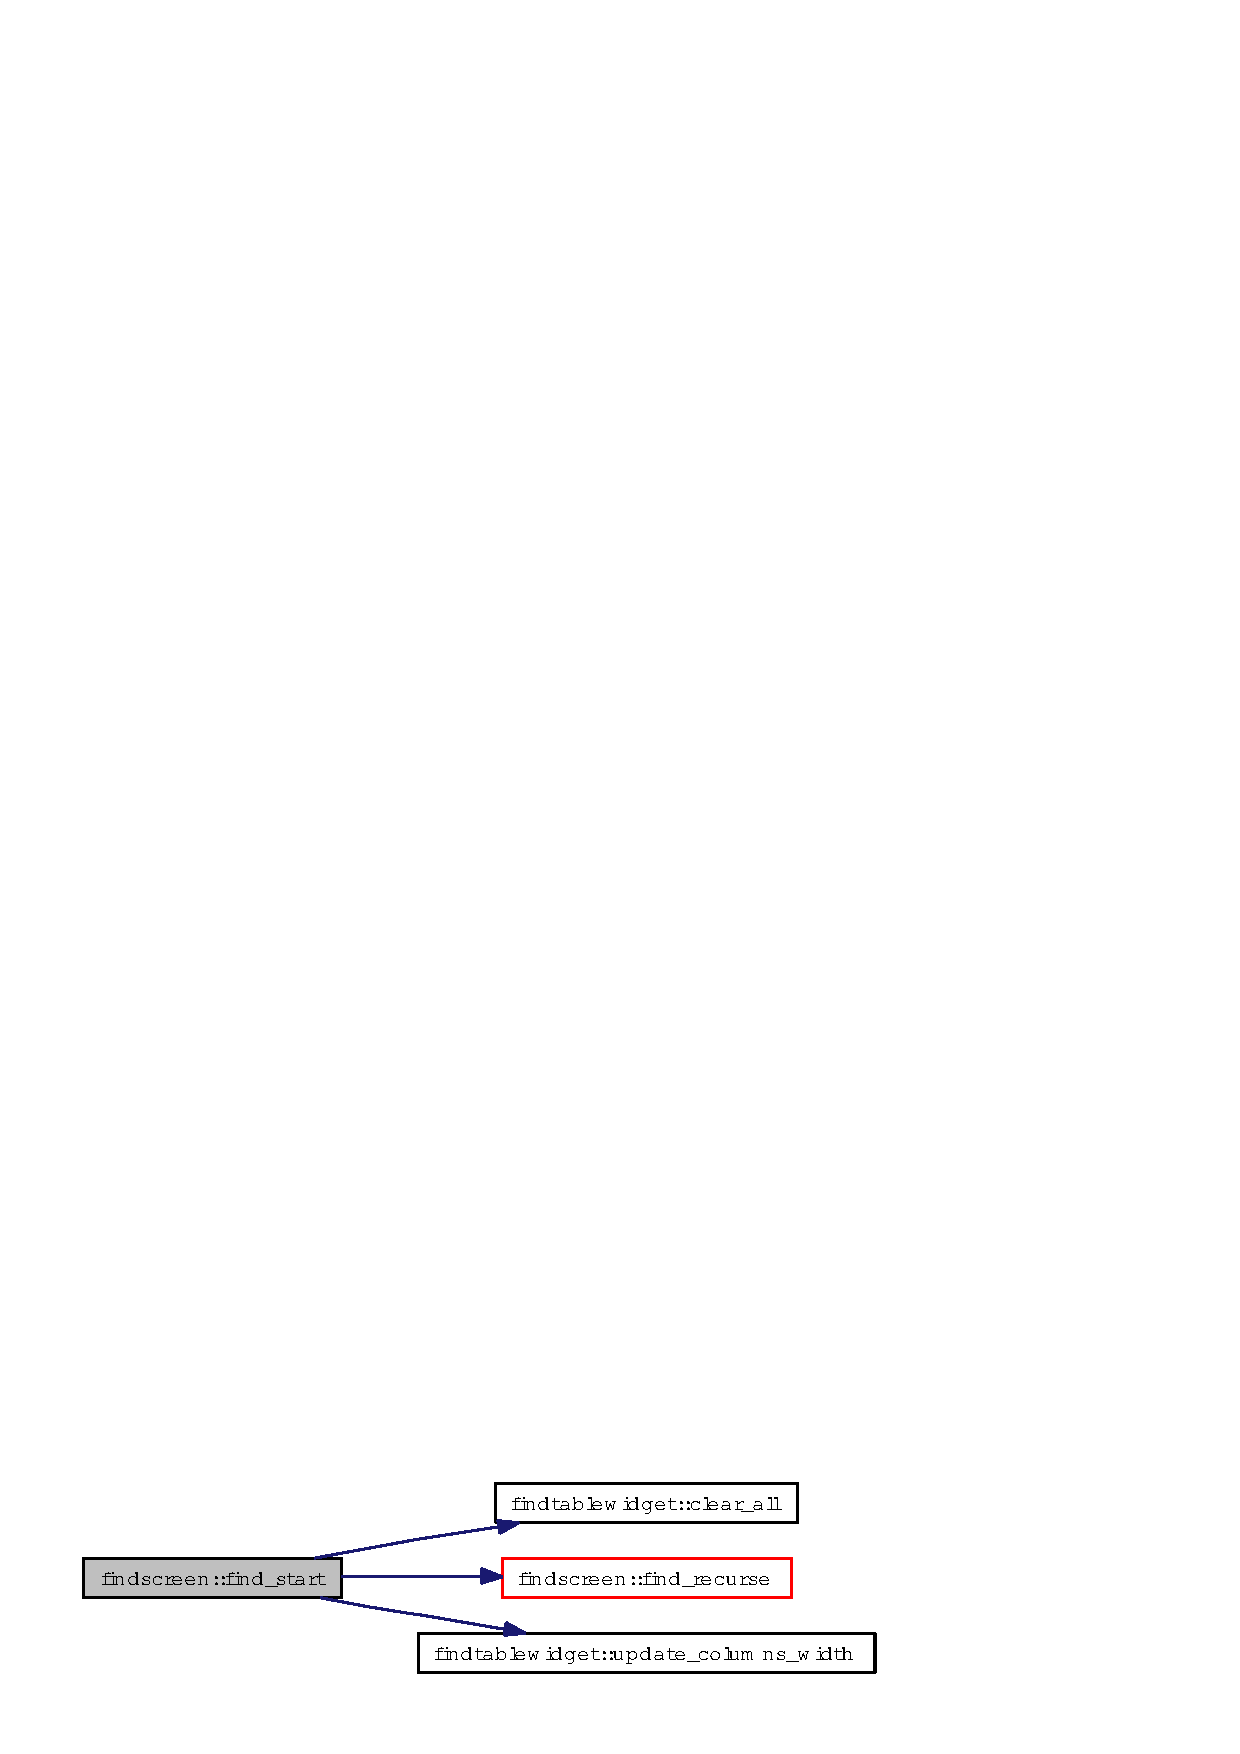
\includegraphics[width=212pt]{classfindscreen_c07d8e7cc43f0ea168768e94d7c83099_cgraph}
\end{center}
\end{figure}
\index{findscreen@{findscreen}!find_recurse@{find\_\-recurse}}
\index{find_recurse@{find\_\-recurse}!findscreen@{findscreen}}
\subsubsection{\setlength{\rightskip}{0pt plus 5cm}void findscreen::find\_\-recurse ({\bf Tree\-Item} $\ast$ {\em curritem})\hspace{0.3cm}{\tt  [private]}}\label{classfindscreen_b962b1004be0e8afb8123a108d9cf73a}




Definition at line 279 of file findscreen.cpp.

References findtablewidget::add\_\-row(), Tree\-Item::child(), Tree\-Item::child\-Count(), Tree\-Item::data(), find\_\-in\_\-text\_\-process(), findtable, Tree\-Item::get\_\-path(), Tree\-Item::recordtable\_\-getrowcount(), Tree\-Item::recordtable\_\-gettabledata(), and search\_\-area.

Referenced by find\_\-start().

Here is the call graph for this function:\begin{figure}[H]
\begin{center}
\leavevmode
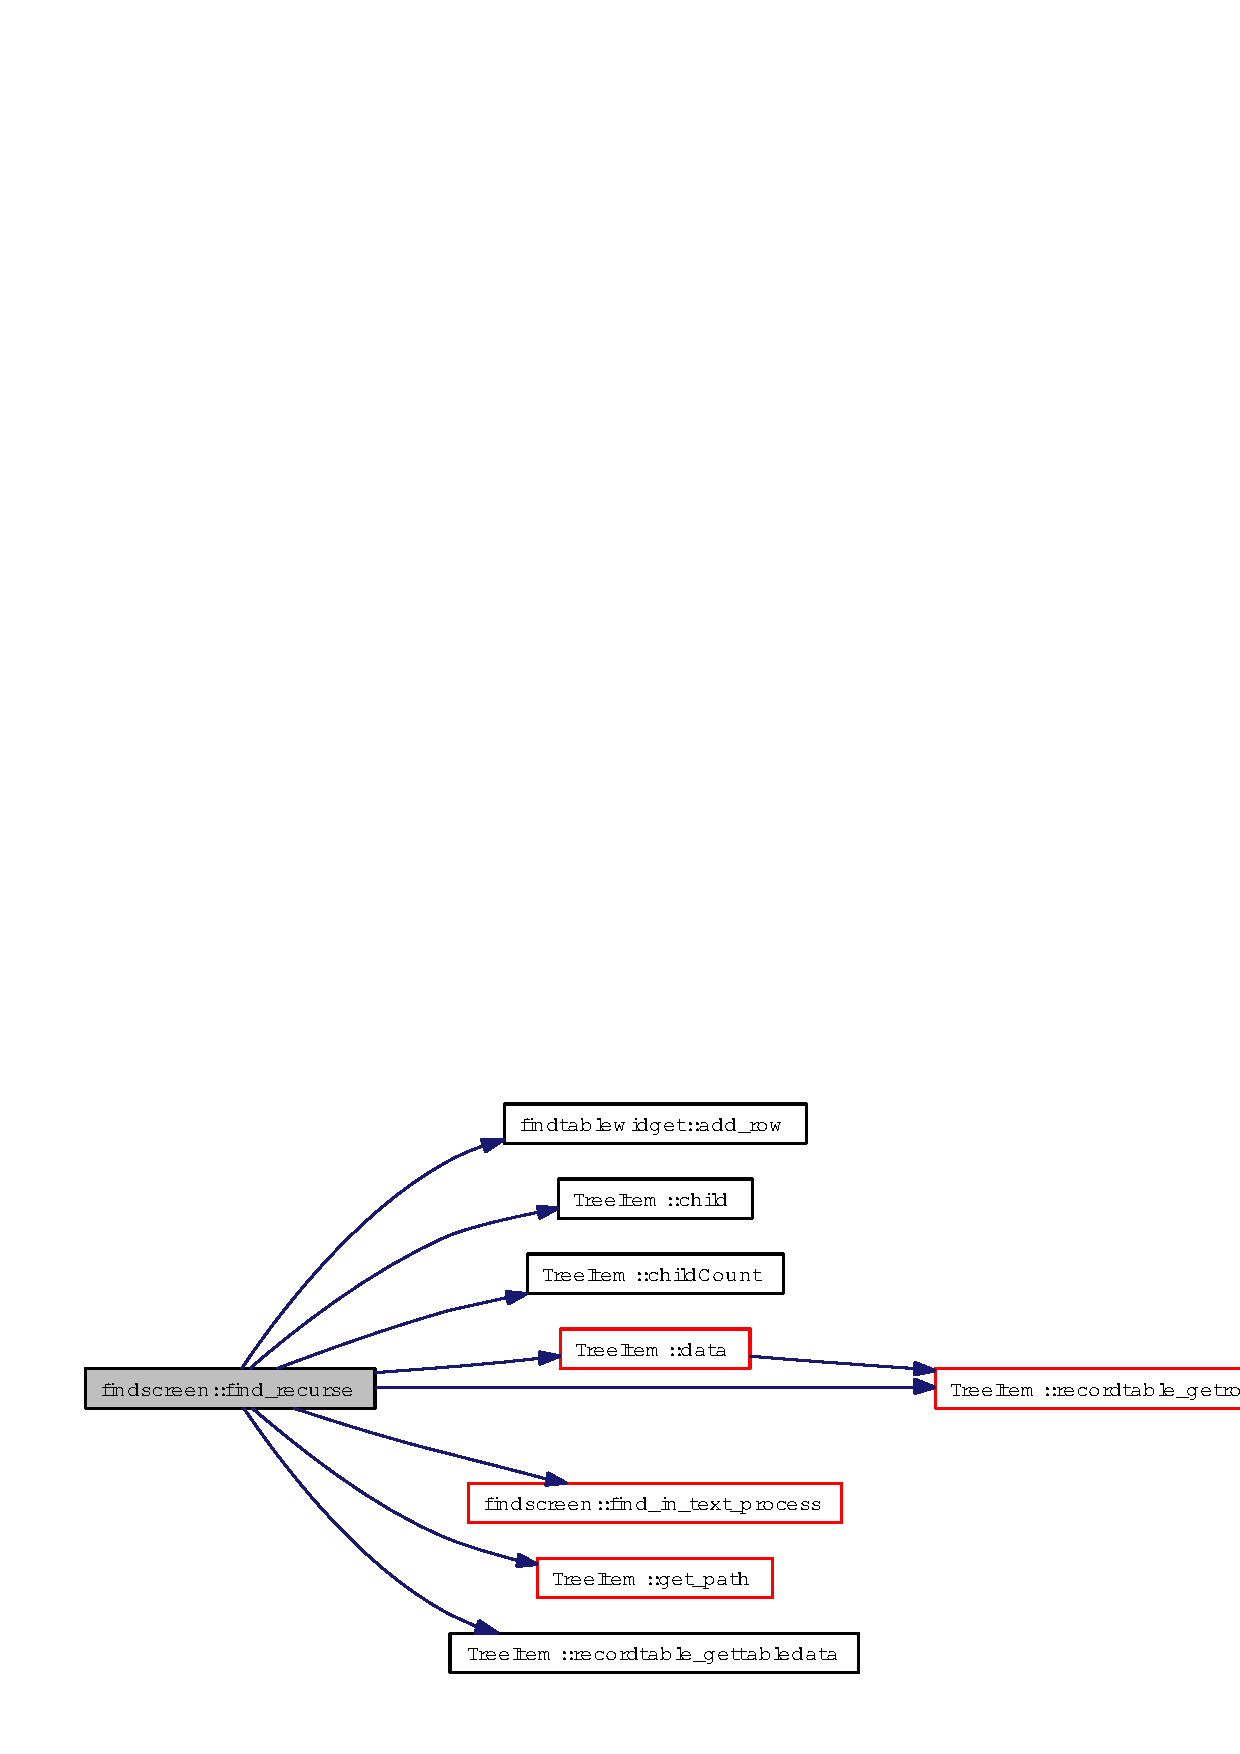
\includegraphics[width=324pt]{classfindscreen_b962b1004be0e8afb8123a108d9cf73a_cgraph}
\end{center}
\end{figure}


Here is the caller graph for this function:\begin{figure}[H]
\begin{center}
\leavevmode
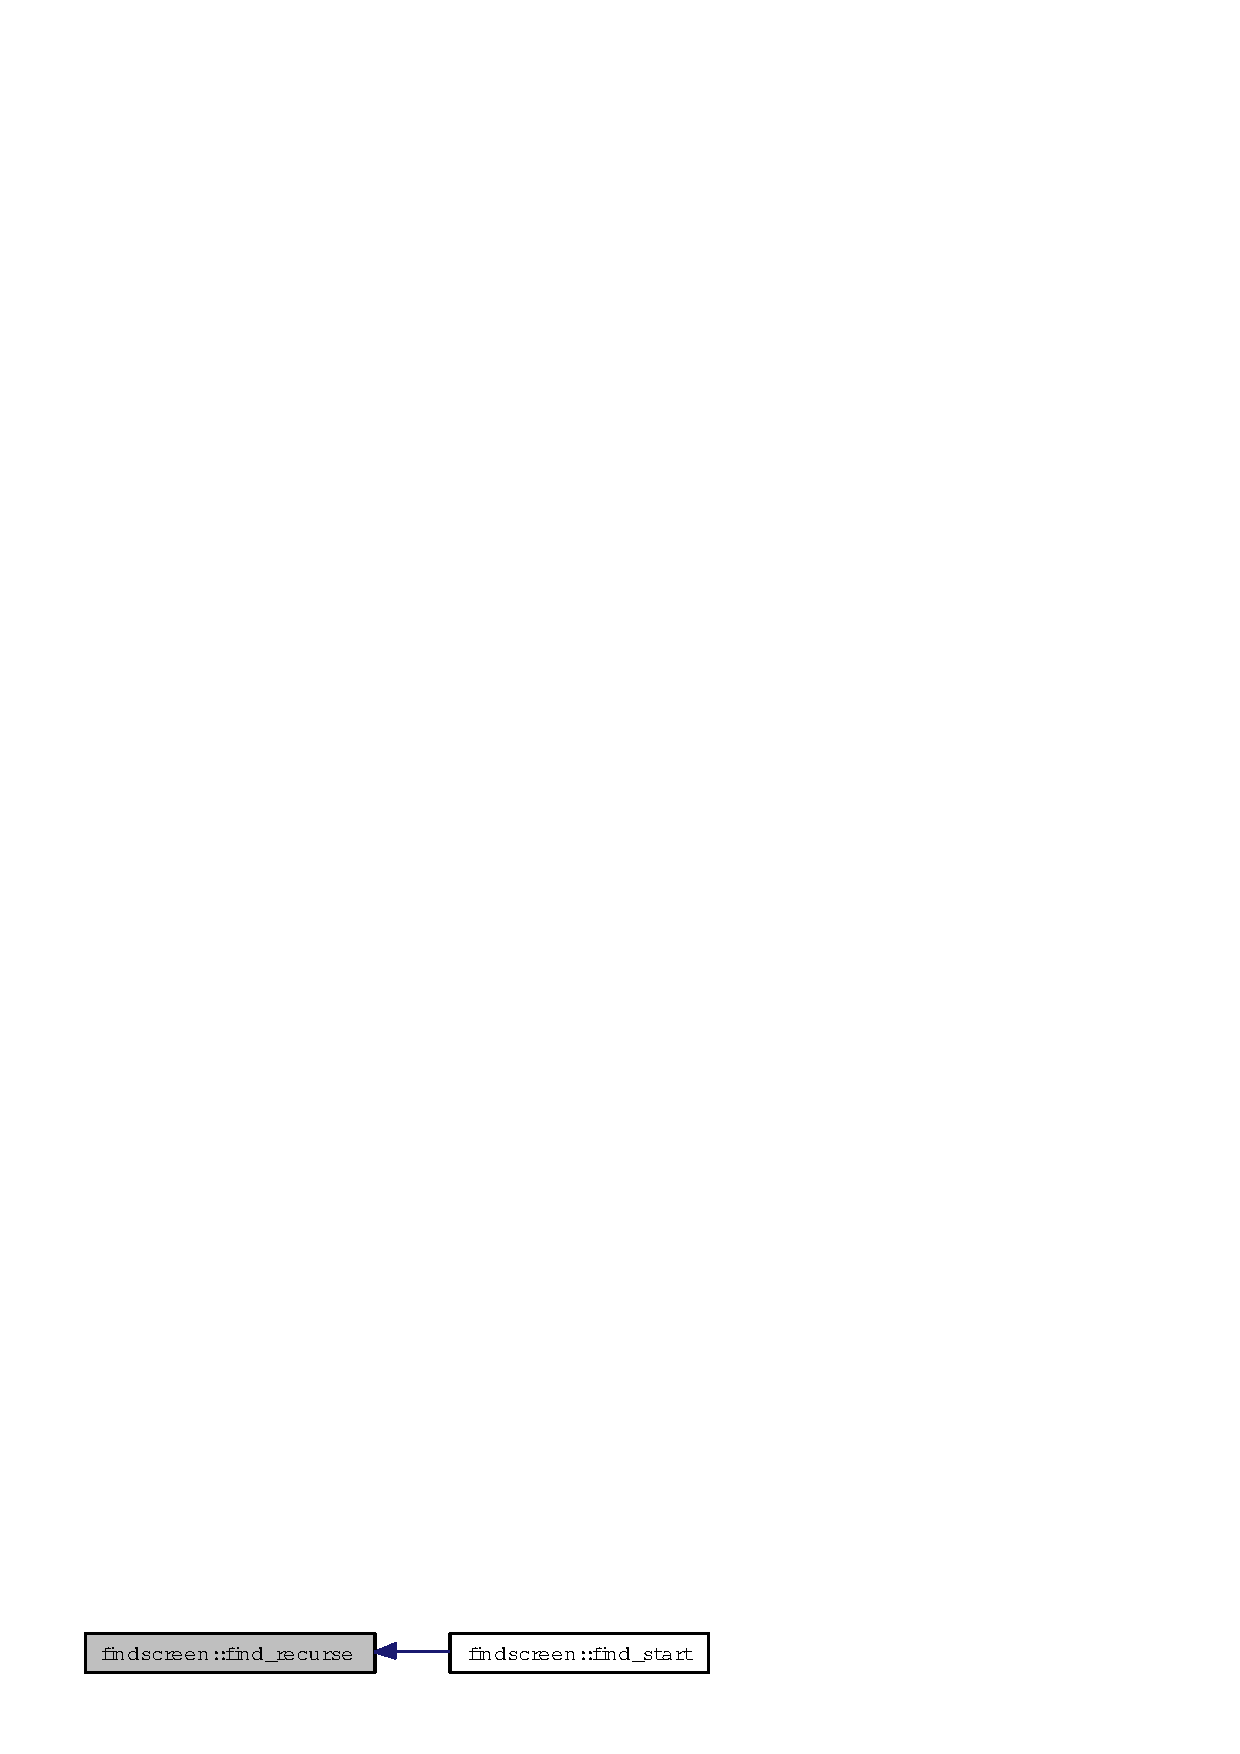
\includegraphics[width=172pt]{classfindscreen_b962b1004be0e8afb8123a108d9cf73a_icgraph}
\end{center}
\end{figure}
\index{findscreen@{findscreen}!text_decompose@{text\_\-decompose}}
\index{text_decompose@{text\_\-decompose}!findscreen@{findscreen}}
\subsubsection{\setlength{\rightskip}{0pt plus 5cm}QString\-List findscreen::text\_\-decompose (QString {\em text})\hspace{0.3cm}{\tt  [private]}}\label{classfindscreen_b5b73fe86f25f27694aabb126539f8f2}




Definition at line 245 of file findscreen.cpp.

Referenced by find\_\-clicked(), and find\_\-in\_\-text\_\-process().

Here is the caller graph for this function:\begin{figure}[H]
\begin{center}
\leavevmode
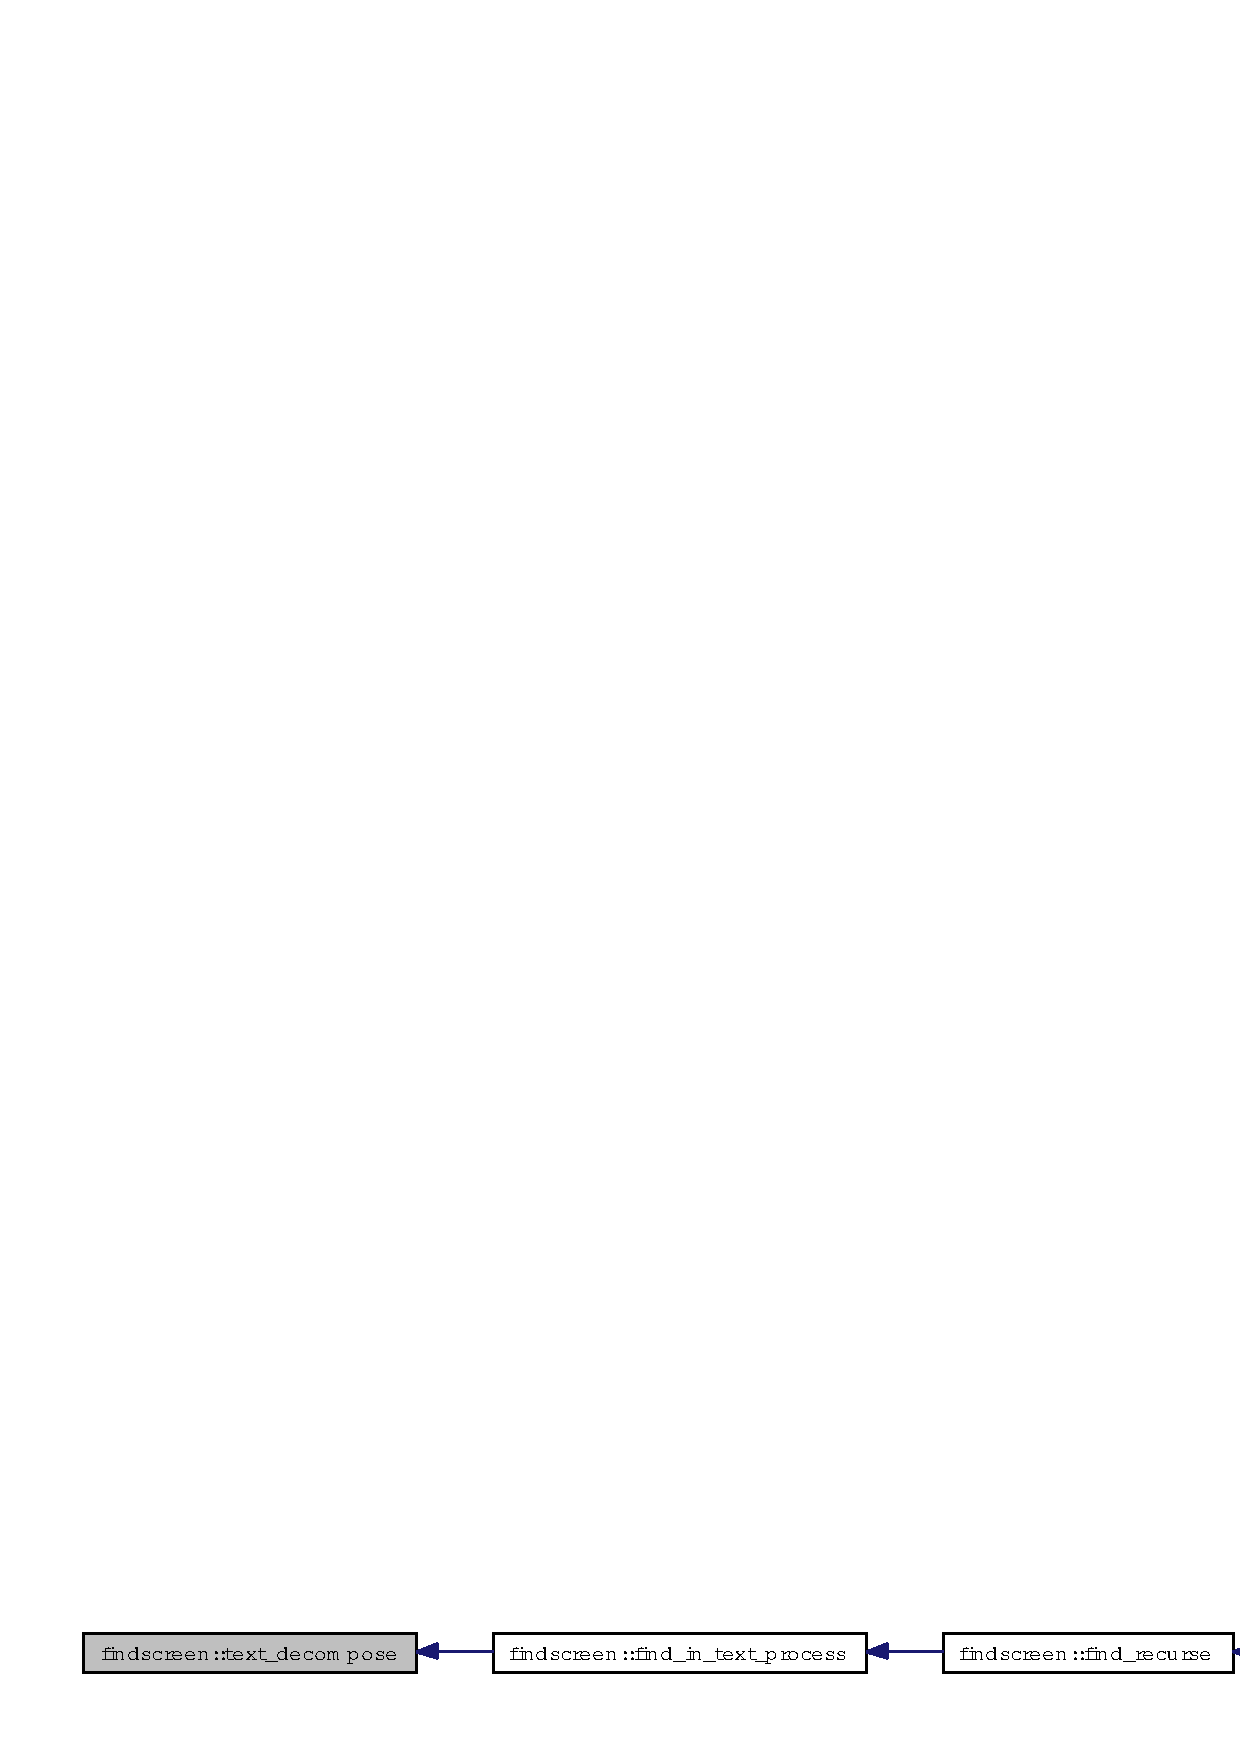
\includegraphics[width=378pt]{classfindscreen_b5b73fe86f25f27694aabb126539f8f2_icgraph}
\end{center}
\end{figure}
\index{findscreen@{findscreen}!find_in_text_process@{find\_\-in\_\-text\_\-process}}
\index{find_in_text_process@{find\_\-in\_\-text\_\-process}!findscreen@{findscreen}}
\subsubsection{\setlength{\rightskip}{0pt plus 5cm}bool findscreen::find\_\-in\_\-text\_\-process (const QString \& {\em text})\hspace{0.3cm}{\tt  [private]}}\label{classfindscreen_d23331d7a6cfd344c12f876fc8e93e31}




Definition at line 368 of file findscreen.cpp.

References howextract, search\_\-word\_\-list, text\_\-decompose(), and wordregard.

Referenced by find\_\-recurse().

Here is the call graph for this function:\begin{figure}[H]
\begin{center}
\leavevmode
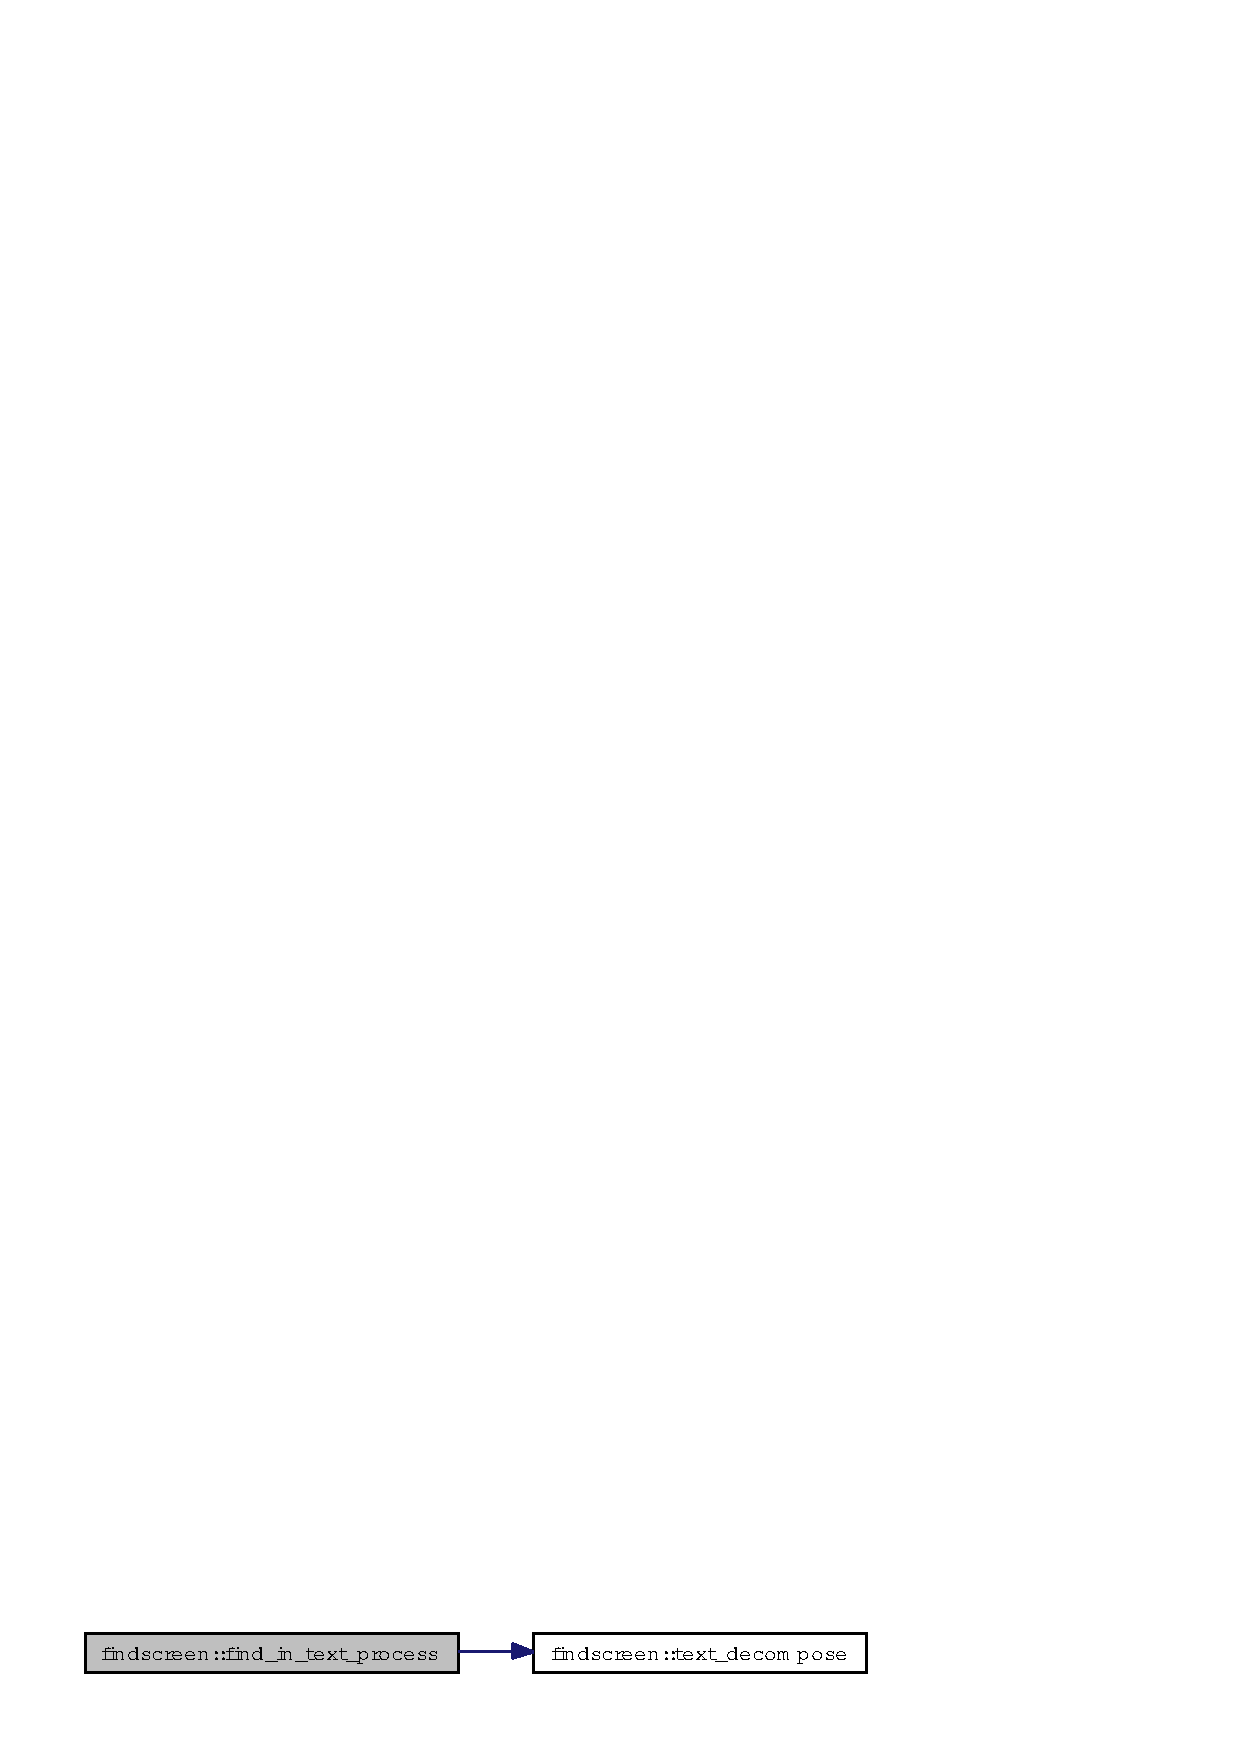
\includegraphics[width=210pt]{classfindscreen_d23331d7a6cfd344c12f876fc8e93e31_cgraph}
\end{center}
\end{figure}


Here is the caller graph for this function:\begin{figure}[H]
\begin{center}
\leavevmode
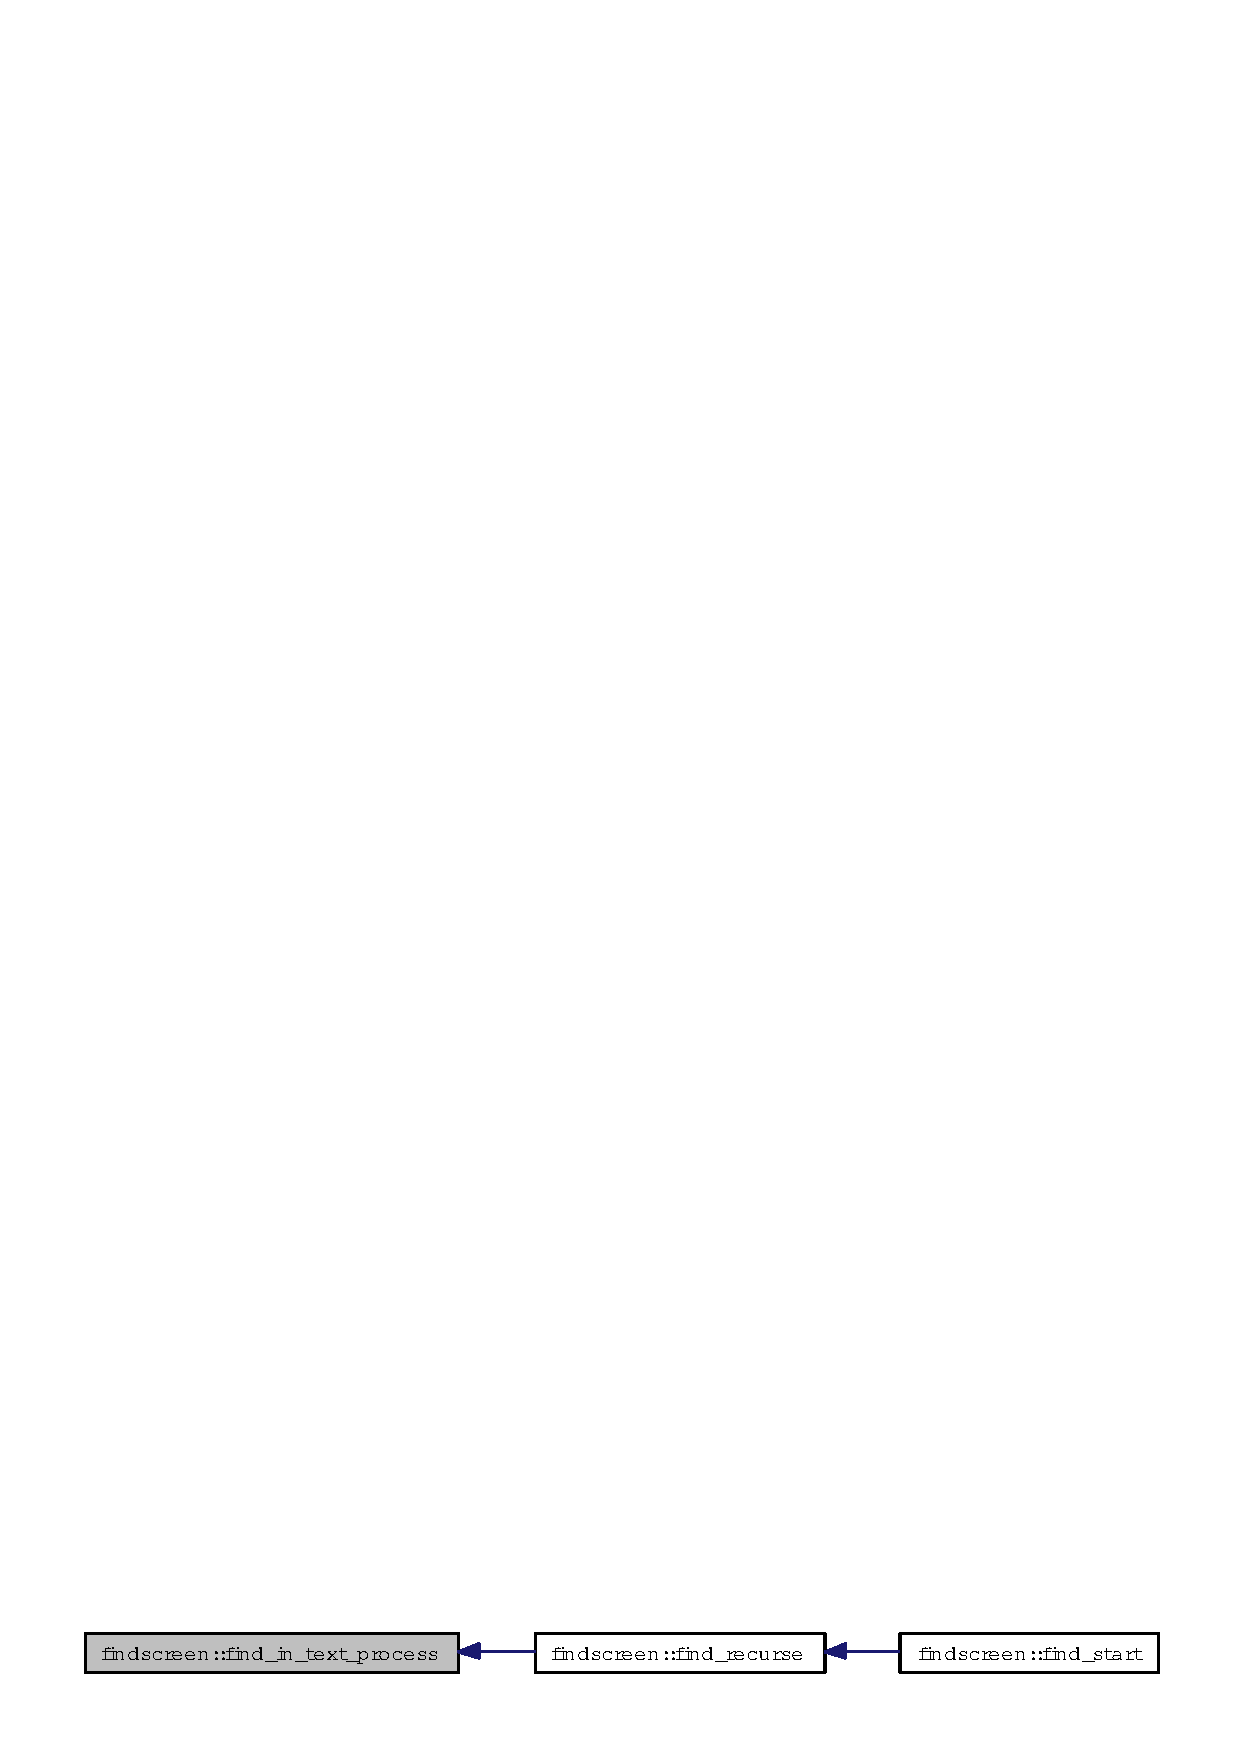
\includegraphics[width=280pt]{classfindscreen_d23331d7a6cfd344c12f876fc8e93e31_icgraph}
\end{center}
\end{figure}


\subsection{Member Data Documentation}
\index{findscreen@{findscreen}!findtext@{findtext}}
\index{findtext@{findtext}!findscreen@{findscreen}}
\subsubsection{\setlength{\rightskip}{0pt plus 5cm}QLine\-Edit$\ast$ {\bf findscreen::findtext}\hspace{0.3cm}{\tt  [private]}}\label{classfindscreen_c25b87182f109dfaf2a7637388792e3d}




Definition at line 47 of file findscreen.h.

Referenced by assembly\_\-toolsline(), find\_\-clicked(), setup\_\-signals(), and setup\_\-toolsline().\index{findscreen@{findscreen}!findstart@{findstart}}
\index{findstart@{findstart}!findscreen@{findscreen}}
\subsubsection{\setlength{\rightskip}{0pt plus 5cm}QPush\-Button$\ast$ {\bf findscreen::findstart}\hspace{0.3cm}{\tt  [private]}}\label{classfindscreen_47c5f30908e29b78cfb6c3976ac7a29e}




Definition at line 48 of file findscreen.h.

Referenced by assembly\_\-toolsline(), enable\_\-find\_\-button(), setup\_\-signals(), and setup\_\-toolsline().\index{findscreen@{findscreen}!wordregard@{wordregard}}
\index{wordregard@{wordregard}!findscreen@{findscreen}}
\subsubsection{\setlength{\rightskip}{0pt plus 5cm}QCombo\-Box$\ast$ {\bf findscreen::wordregard}\hspace{0.3cm}{\tt  [private]}}\label{classfindscreen_65acfc42865bbda3765bbc573872947c}




Definition at line 49 of file findscreen.h.

Referenced by assembly\_\-toolsline(), find\_\-in\_\-text\_\-process(), setup\_\-signals(), and setup\_\-toolsline().\index{findscreen@{findscreen}!howextract@{howextract}}
\index{howextract@{howextract}!findscreen@{findscreen}}
\subsubsection{\setlength{\rightskip}{0pt plus 5cm}QCombo\-Box$\ast$ {\bf findscreen::howextract}\hspace{0.3cm}{\tt  [private]}}\label{classfindscreen_93a56ea65a506789dc79973c2a0c7b4f}




Definition at line 50 of file findscreen.h.

Referenced by assembly\_\-toolsline(), find\_\-in\_\-text\_\-process(), setup\_\-signals(), and setup\_\-toolsline().\index{findscreen@{findscreen}!closebutton@{closebutton}}
\index{closebutton@{closebutton}!findscreen@{findscreen}}
\subsubsection{\setlength{\rightskip}{0pt plus 5cm}QTool\-Button$\ast$ {\bf findscreen::closebutton}\hspace{0.3cm}{\tt  [private]}}\label{classfindscreen_f09efcdef871da758f4781430a5387d0}




Definition at line 51 of file findscreen.h.

Referenced by assembly\_\-toolsline(), setup\_\-signals(), and setup\_\-toolsline().\index{findscreen@{findscreen}!wherefindlabel@{wherefindlabel}}
\index{wherefindlabel@{wherefindlabel}!findscreen@{findscreen}}
\subsubsection{\setlength{\rightskip}{0pt plus 5cm}QLabel$\ast$ {\bf findscreen::wherefindlabel}\hspace{0.3cm}{\tt  [private]}}\label{classfindscreen_f9d6d76dc6bbdc944680b4cb9a17fd60}




Definition at line 53 of file findscreen.h.

Referenced by assembly\_\-wherefindline(), and setup\_\-wherefindline().\index{findscreen@{findscreen}!find_in_name@{find\_\-in\_\-name}}
\index{find_in_name@{find\_\-in\_\-name}!findscreen@{findscreen}}
\subsubsection{\setlength{\rightskip}{0pt plus 5cm}QCheck\-Box$\ast$ {\bf findscreen::find\_\-in\_\-name}\hspace{0.3cm}{\tt  [private]}}\label{classfindscreen_78c21b2cd74345259c68d8e8590a4643}




Definition at line 54 of file findscreen.h.

Referenced by assembly\_\-wherefindline(), find\_\-clicked(), setup\_\-signals(), and setup\_\-wherefindline().\index{findscreen@{findscreen}!find_in_author@{find\_\-in\_\-author}}
\index{find_in_author@{find\_\-in\_\-author}!findscreen@{findscreen}}
\subsubsection{\setlength{\rightskip}{0pt plus 5cm}QCheck\-Box$\ast$ {\bf findscreen::find\_\-in\_\-author}\hspace{0.3cm}{\tt  [private]}}\label{classfindscreen_477073cf51add2711594bc0210ad4384}




Definition at line 55 of file findscreen.h.

Referenced by assembly\_\-wherefindline(), find\_\-clicked(), setup\_\-signals(), and setup\_\-wherefindline().\index{findscreen@{findscreen}!find_in_url@{find\_\-in\_\-url}}
\index{find_in_url@{find\_\-in\_\-url}!findscreen@{findscreen}}
\subsubsection{\setlength{\rightskip}{0pt plus 5cm}QCheck\-Box$\ast$ {\bf findscreen::find\_\-in\_\-url}\hspace{0.3cm}{\tt  [private]}}\label{classfindscreen_b1e5580091a5e4dfaf77e0c08b86ac9a}




Definition at line 56 of file findscreen.h.

Referenced by assembly\_\-wherefindline(), find\_\-clicked(), setup\_\-signals(), and setup\_\-wherefindline().\index{findscreen@{findscreen}!find_in_tags@{find\_\-in\_\-tags}}
\index{find_in_tags@{find\_\-in\_\-tags}!findscreen@{findscreen}}
\subsubsection{\setlength{\rightskip}{0pt plus 5cm}QCheck\-Box$\ast$ {\bf findscreen::find\_\-in\_\-tags}\hspace{0.3cm}{\tt  [private]}}\label{classfindscreen_278085c269b591f3f21dc8d9b3bbeb36}




Definition at line 57 of file findscreen.h.

Referenced by assembly\_\-wherefindline(), find\_\-clicked(), setup\_\-signals(), and setup\_\-wherefindline().\index{findscreen@{findscreen}!find_in_text@{find\_\-in\_\-text}}
\index{find_in_text@{find\_\-in\_\-text}!findscreen@{findscreen}}
\subsubsection{\setlength{\rightskip}{0pt plus 5cm}QCheck\-Box$\ast$ {\bf findscreen::find\_\-in\_\-text}\hspace{0.3cm}{\tt  [private]}}\label{classfindscreen_39e9062c690996843f63688123d3bb3e}




Definition at line 58 of file findscreen.h.

Referenced by assembly\_\-wherefindline(), find\_\-clicked(), setup\_\-signals(), and setup\_\-wherefindline().\index{findscreen@{findscreen}!toolsline@{toolsline}}
\index{toolsline@{toolsline}!findscreen@{findscreen}}
\subsubsection{\setlength{\rightskip}{0pt plus 5cm}QHBox\-Layout$\ast$ {\bf findscreen::toolsline}\hspace{0.3cm}{\tt  [private]}}\label{classfindscreen_fa5c4d3189d40d76b66bd7cc027d0aa0}




Definition at line 60 of file findscreen.h.

Referenced by assembly(), and assembly\_\-toolsline().\index{findscreen@{findscreen}!placeupclosebutton@{placeupclosebutton}}
\index{placeupclosebutton@{placeupclosebutton}!findscreen@{findscreen}}
\subsubsection{\setlength{\rightskip}{0pt plus 5cm}QVBox\-Layout$\ast$ {\bf findscreen::placeupclosebutton}\hspace{0.3cm}{\tt  [private]}}\label{classfindscreen_7036a96e3ee8e35c3fc1e50923f28e68}




Definition at line 61 of file findscreen.h.

Referenced by assembly\_\-toolsline().\index{findscreen@{findscreen}!wherefindline@{wherefindline}}
\index{wherefindline@{wherefindline}!findscreen@{findscreen}}
\subsubsection{\setlength{\rightskip}{0pt plus 5cm}QHBox\-Layout$\ast$ {\bf findscreen::wherefindline}\hspace{0.3cm}{\tt  [private]}}\label{classfindscreen_25386ff1d160154580941a0cba4d9e8f}




Definition at line 62 of file findscreen.h.

Referenced by assembly(), and assembly\_\-wherefindline().\index{findscreen@{findscreen}!centrallayout@{centrallayout}}
\index{centrallayout@{centrallayout}!findscreen@{findscreen}}
\subsubsection{\setlength{\rightskip}{0pt plus 5cm}QVBox\-Layout$\ast$ {\bf findscreen::centrallayout}\hspace{0.3cm}{\tt  [private]}}\label{classfindscreen_6f77f9b004aa58ea1555cade0ea5bbcd}




Definition at line 63 of file findscreen.h.

Referenced by assembly().\index{findscreen@{findscreen}!findtable@{findtable}}
\index{findtable@{findtable}!findscreen@{findscreen}}
\subsubsection{\setlength{\rightskip}{0pt plus 5cm}{\bf findtablewidget}$\ast$ {\bf findscreen::findtable}\hspace{0.3cm}{\tt  [private]}}\label{classfindscreen_b51326b828689313939e3aca6a224f10}




Definition at line 65 of file findscreen.h.

Referenced by assembly(), find\_\-recurse(), find\_\-start(), and setup\_\-ui().\index{findscreen@{findscreen}!search_area@{search\_\-area}}
\index{search_area@{search\_\-area}!findscreen@{findscreen}}
\subsubsection{\setlength{\rightskip}{0pt plus 5cm}QMap$<$QString, bool$>$ {\bf findscreen::search\_\-area}\hspace{0.3cm}{\tt  [private]}}\label{classfindscreen_f79593d8e31d6434bcc842cec63e48b3}




Definition at line 86 of file findscreen.h.

Referenced by find\_\-clicked(), and find\_\-recurse().\index{findscreen@{findscreen}!search_word_list@{search\_\-word\_\-list}}
\index{search_word_list@{search\_\-word\_\-list}!findscreen@{findscreen}}
\subsubsection{\setlength{\rightskip}{0pt plus 5cm}QString\-List {\bf findscreen::search\_\-word\_\-list}\hspace{0.3cm}{\tt  [private]}}\label{classfindscreen_48e985c7f0fafaa386a5708c45395a75}




Definition at line 89 of file findscreen.h.

Referenced by find\_\-clicked(), and find\_\-in\_\-text\_\-process().

The documentation for this class was generated from the following files:\begin{CompactItemize}
\item 
{\bf findscreen.h}\item 
{\bf findscreen.cpp}\end{CompactItemize}
